
\usepackage{minted}


\usepackage{xcolor}
\usepackage{colortbl}

\usepackage{fontspec}
\setmainfont{Linux Libertine O}
\usepackage{xltxtra}
\usepackage[english,french]{babel}


\def\exampleFont{\ttfamily\small}

\usepackage{framed}
\definecolor{shadecolor}{gray}{0.95}
\usepackage{longtable}
\usepackage[normalem]{ulem}

\institute{Univ. de Neuchâtel}

\title{Introduction}
\subtitle{Philologie numérique et édition électronique}
\author{Jean-Baptiste Camps \& Simon Gabay}
\date[FoPhil -- 12 févr. 2018]{Formation en philologie numérique:\\ encoder, exploiter, diffuser\\
12-16 février 2018}

\makeatletter 
         
        \AtBeginSection[]{% 
        \begin{frame}{Plan}%
        \small
        \tableofcontents[currentsection]%
        \end{frame} }

        %\AtBeginSubsection[]{% 
	%\begin{frame}{Plan}%
	%\small
	%\tableofcontents[currentsection,currentsubsection]%
%\end{frame} }


\makeatother 
    
\newcommand{\orgName}{\scshape}
    
\begin{document}

\frame{\maketitle}

%\frontmatter 
  

%\mainmatter 


\begin{frame}
\frametitle{Philologie numérique} %, philologie des données}
    
    \begin{block}{\textit{digital approach to philology} \cite{Andrews2012}}
     \alert{L'emploi de méthodes computationnelles à toutes les étapes du travail philologique}, de la \emph{production} des données (recension, transcription, collation, …) à leur \emph{analyse}.
    \end{block}
    
    \begin{block}{Philologie tournée vers les données}
     une approche qui mette \alert{les données au centre}:
     \begin{description}
     \item[en amont] tirer profit des méthodes computationnelles pour produire des données dans des quantités ou granularités jusque là inenvisageables.% (reconnaissance des écritures manuscrites, annotation linguistique, collation assistée par ordinateur…);
     \item[en aval] partir des données plutôt que de leur plaquer des hypothèses préexistantes.
     \item[au centre] les \emph{données} elles-mêmes, formalisées selon un \emph{modèle} représentant les faits étudiés, et accessibles de manière \emph{transparente}.
     \end{description}
    \end{block}
    
\end{frame}

\begin{frame}{Que sont les données pour des philologues?}

\begin{itemize}
    \item \alert{des textes} ou, plus souvent, les \alert{témoins} de textes, conservés notamment dans des manuscrits;
    \item ayant fait l'objet d'un travail philologique d'\alert{édition};
    \item \alert{enrichis} par l'expertise ou l'interprétation philologique (annotation, interprétation,…)
\end{itemize}

\begin{block}{Problèmes}

\begin{itemize}
    \item Comment rendre ce travail (interprétatif) philologique le plus \emph{transparent} possible?
    \item Comment rendre ces données \emph{réutilisables} par d'autres?
    \item Comment favoriser les nouveaux questionnements, les nouvelles enquêtes, les nouvelles utilisations de nos données?
\end{itemize}
 
\end{block}

\end{frame}

\begin{frame}
\frametitle{Philologie numérique, science des données, science ouverte}
    
    \begin{columns}
    \begin{column}{0.60\textwidth}
    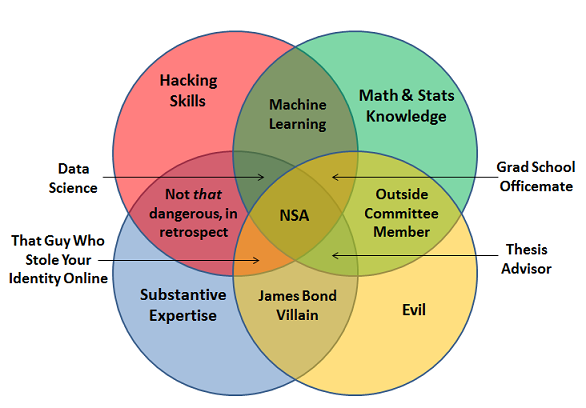
\includegraphics[width=\textwidth]{images/VennDiagram2.png}
    
    {\tiny Source: %Joel Grus, « Post-Prism Data Science Venn Diagram », 9 juin 2013, \url{http://joelgrus.com/2013/06/09/post-prism-data-science-venn-diagram/}, repris par 
    Elijah Meeks, \og{}Digital Humanities and Data Science\fg{}, \textit{Stanford Digital Humanities}, 2014, \url{https://digitalhumanities.stanford.edu/digital-humanities-and-data-science}.}
    \end{column}
    \begin{column}{0.40\textwidth}
    \textsc{Avantages}
    \begin{itemize}
        \item nouvelles données, nouveaux questionnements;
        \item cumulabilité;
        \item reproductibilité;
        \item réfutabilité.
    \end{itemize}
    \end{column}
    \end{columns}
    
\end{frame}

\begin{frame}{\textsc{Fair} Data}
%Cf. les principes soutenus par les États et agences de recherche (CE, ERC,…)
\begin{center}

\includegraphics[width=0.6\textwidth]{images/FAIR_data_principles.jpg}
    
    {\footnotesize (Img. SangyaPundir CC BY-SA 4.0)}%, \url{https://commons.wikimedia.org/w/index.php?curid=53414062}}
\end{center}

\begin{columns}[T]
    \begin{column}{0.5\textwidth}
\begin{itemize}
        \item \textit{Findable}: données doivent être faciles à trouver en ligne, y compris sur le long terme (archivage pérenne);% provinding persistents identifier. 
        \item \textit{Accessible}: format ouvert, libre, documenté et compréhensible;
\end{itemize}
    \end{column}
    \begin{column}{0.5\textwidth}
         \begin{itemize}
        \item \textit{Interoperable}: pas enfermées dans un logiciel propriétaire; standards, intégrité des données, documentation;
        \item \textit{Reusable}: données ouvertes, réutilisables  (légalement, techniquement,…).
    \end{itemize}
    \end{column}
\end{columns}


\end{frame}

\begin{frame} 
  \frametitle{Plan} 
  \tableofcontents
\end{frame}

\section{Qu'est-ce qu'une édition électronique?}
\begin{frame}
\frametitle{Intuition}
\begin{itemize}
\item Un ensemble de fichiers électroniques,
\item encodés de manière sémantique, en XML (XML/TEI),
\item publiés sous forme de page web,
\item et plutôt sur un site institutionnel.
\end{itemize} 

  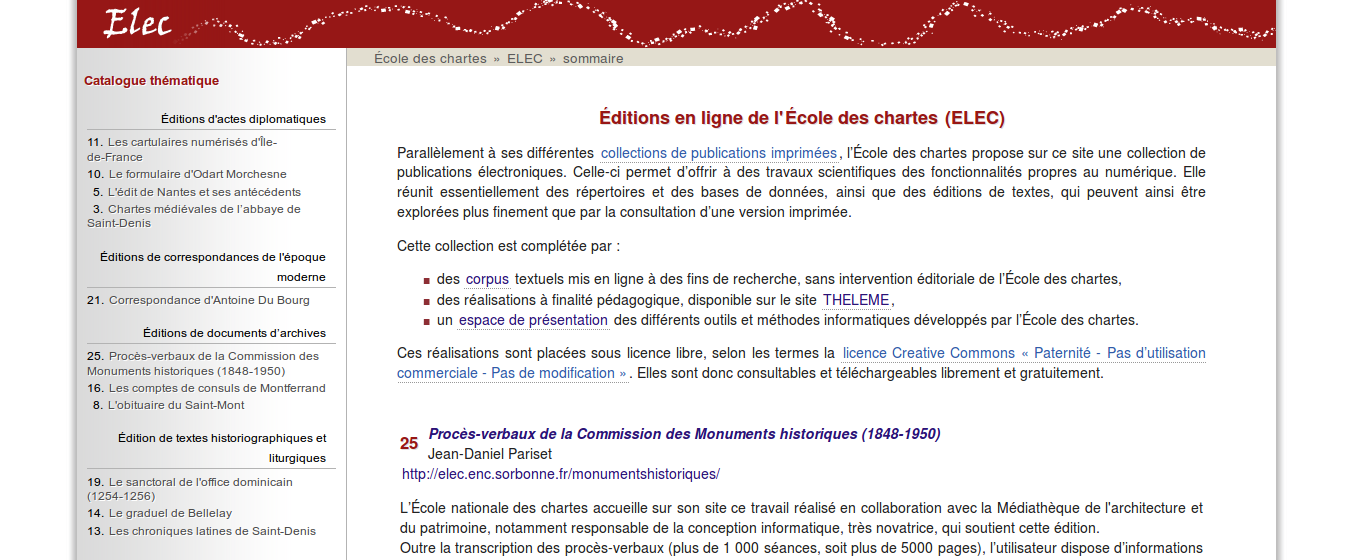
\includegraphics[width=\textwidth]{images/ELEC_accueil.png}
  
\textit{Page d'accueil des Éditions en ligne de l'École des chartes (ÉLEC)}
\end{frame}

\begin{frame}[fragile,squeeze]
\frametitle{Définition minimaliste}{}

 \begin{block}{Édition électronique} Une édition qui fait appel, à un stade ou un autre de sa réalisation (établissement du texte et des index, analyse historique, linguistique ou littéraire et commentaire, publication, diffusion…) au medium électronique. 
 \end{block} 
\end{frame}

\begin{frame}[shrink]
\frametitle{Qu'est-ce qu'une édition qui \textit{n'est pas} électronique?}

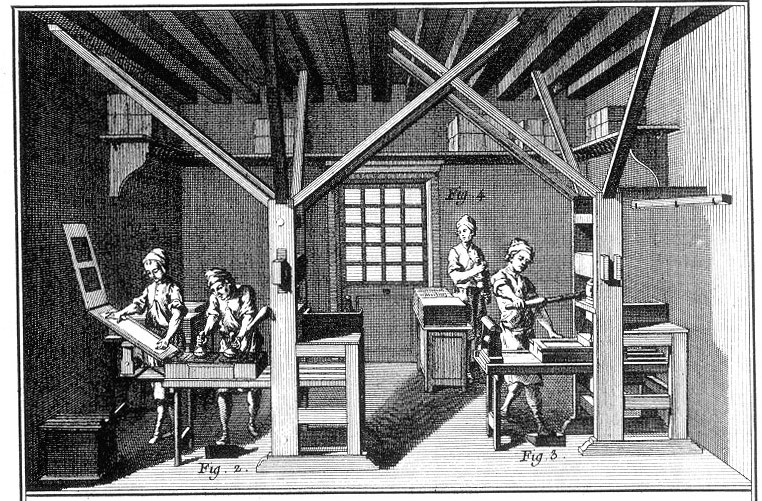
\includegraphics[width=\textwidth]{images/presse.jpeg}
  
\textit{Encyclopédie, art. «Imprimerie»}
\end{frame}

\begin{frame}
\frametitle{Nouvelle définition}

  \begin{block}{Édition électronique} Une édition dont la forme finale est constituée de fichiers électroniques, et qui est diffusée sous cette forme, soit par un réseau (Internet,...), soit sur un support de stockage (CD, ...). \end{block} \begin{itemize}

\item Une page html statique est-elle une édition électronique?
\item Un fichier pdf ou Open Document constitue-t-il une édition électronique?
\item Un ensemble de fichiers de texte mis à disposition constitue-t-il une édition électronique?
\end{itemize} 
\end{frame}

\begin{frame}[shrink]
\frametitle{Édition numérisée ou numérique?}

\begin{block}{numérisée vs. numérique \cite{Sahle2008}} distinction entre \textbf{édition numérisée} (imprimée à l'écran) et \textbf{édition numérique}, i.e., \textit{une édition qui ne peut être imprimée sans perte d'information, dont les fonctionnalités ne sont pas entièrement reproductibles par une version imprimée}. 
\end{block}  


\begin{quotation}
	Digital scholarly editions are not just scholarly editions in digital media. I distinguish between digital and digitized. A digitized print edition is not a « digital edition » in the strict sense used here. A digital edition can not be printed without a loss of information and/or functionality. The digital edition is guided by a different paradigm. If the paradigm of an edition is limited to the two-dimensional space of the « page » and to typographic means of information representation, then it's not a digital edition
\end{quotation}

\end{frame}

\begin{frame}{Édition électronique savante / critique}


\begin{block}{Édition électronique savante (Digital scholarly edition)} 
Une édition qui utilise les possibilités de l'outil informatique pour proposer
\begin{itemize}
	\item une \textbf{représentation critique ou enrichie sémantiquement} d'une source;
	\item des fonctionnalités utiles à leur compréhension et leur analyse.
\end{itemize}
\end{block}  

%\begin{block}{Édition électronique savante (Digital scholarly
%                                edition)} Une édition qui explicite la structure et le sémantisme d'un certain nombre de phénomènes propres au texte ou à la source pour en permettre le traitement par un ordinateur.  
%\end{block} 

\end{frame}


\section[Principes et fondamentaux]{Principes et fondamentaux de l'édition électronique}
\subsection{Comment représenter un texte?}

\begin{frame}[fragile]
\frametitle{Comment représenter un texte?}{}
\begin{block}{}
On emploie \emph{a priori} les italiques pour les locutions et termes empruntés à d’autres langues.
\end{block}
\end{frame}

\begin{frame}[fragile]
\frametitle{Deux approches possibles}\begin{block}{}On emploie \textit{a priori} les italiques pour les locutions et termes empruntés à d’autres langues.\end{block}
        \bgroup\ttfamily\fontsize{8.5pt}{9pt}\selectfont

        \begin{exampleblock}{Procédural}
        \noindent\ttfamily\mbox{} On emploie\mbox{}\newline 
 /ici commence un texte en italiques/ a priori /ici finit un texte en\mbox{}\newline 
 italiques/ les italiques... 
        \end{exampleblock}
        
\egroup
    
        \bgroup\ttfamily\fontsize{8.5pt}{9pt}\selectfont

        \begin{exampleblock}{Sémantique}
        \noindent\ttfamily\mbox{} On emploie\mbox{}\newline 
 /ici commence une locution étrangère/ a priori /ici finit une locution\mbox{}\newline 
 étrangère/ les italiques 
        \end{exampleblock}
        
\egroup
    
\end{frame}

%\begin{frame}[fragile]
%\frametitle{Différentes solutions dans différents langages}\begin{block}{}On emploie \textit{a priori} les italiques pour les locutions et termes empruntés à d’autres langues.\end{block}
%    \noindent
%  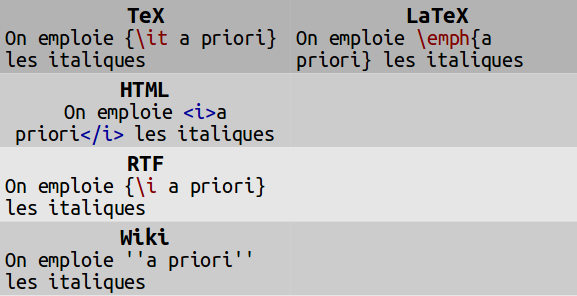
\includegraphics[width=\textwidth]{images/exemplesLangages.png}
%  
%  \textit{Différents balisages dans des langages courants}
%\end{frame}

\begin{frame}[fragile]
\frametitle{Solutions XML}
        \bgroup\ttfamily\fontsize{8.5pt}{9pt}\selectfont

        \begin{exampleblock}{Une solution en XML}
        \noindent\ttfamily\mbox{} On\mbox{}\newline 
 emploie {\color{blue}<\textbf{locutionÉtrangère}>}a priori{\color{blue}</\textbf{locutionÉtrangère}>} les italiques\mbox{}\newline 
 pour les locutions et termes empruntés à d’autres langues. 
        \end{exampleblock}
        
\egroup
    
        \bgroup\ttfamily\fontsize{8.5pt}{9pt}\selectfont

        \begin{exampleblock}{En TEI}
        \noindent\ttfamily\mbox{} On emploie\mbox{}\newline 
{\color{blue}<\textbf{foreign}{\color{blue}{} xml:lang}="{\color{blue}{}la}">}a priori{\color{blue}</\textbf{foreign}>} les italiques… 
        \end{exampleblock}
        
\egroup
    
\end{frame}

\begin{frame}[fragile]
\frametitle{Autres solutions XML}

\ttfamily\fontsize{8.5pt}{9pt}\selectfont

\begin{exampleblock}{Utilisation pédagogique}
\begin{minted}{xml}
<exemple>On emploie <cas>a priori</cas> les italiques
 pour les locutions et termes empruntés 
 à d’autres langues.</exemple>
\end{minted}
\end{exampleblock}

\begin{exampleblock}{Langue et morpho-syntaxe}
\begin{minted}{xml}
<phrase>
  <mot type="pronom" subtype="personnel">On</mot>
  <mot type="verbe" subtype="conjugué">emploie</mot>
  <!-- etc. -->
</phrase>
\end{minted}
\end{exampleblock}

\end{frame}

\begin{frame}
\frametitle{eXtensible (2) Markup Language (1)}\begin{itemize}

\item[1] Le ML de XML : markup language, XML est un langage à balises ;
\item[2] le X de XML : XML est eXtensible (i.e., il ne propose pas un jeu prédéfini et fermé de balises, mais une syntaxe, et des règles sur ce que doit être un document XML bien formé, un document valide et sur l'écriture de grammaires spécifiques).
\end{itemize} 
\end{frame}

\begin{frame}[fragile]
\frametitle{XML comme langage structuré (par des balises)}
        \bgroup\ttfamily\fontsize{8.5pt}{9pt}\selectfont

\begin{minted}{xml}
<document>
  <paragraphe>
    <phrase>
      On emploie <locutionÉtrangère>a priori</locutionÉtrangère> 
      les italiques pour les locutions et termes empruntés 
      à d’autres langues.
    </phrase>
    <phrase>
      On emploie souvent les petites capitales pour les noms propres, 
      comme <nom>Léopold Delisle</nom> ou <nom>Jules Quicherat</nom>.
    </phrase>
    <phrase>
      On emploie en revanche généralement le gras pour des raisons 
      coupables.
    </phrase>
  </paragraphe>
  <paragraphe>
    <phrase>
      Un second paragraphe...
    </phrase>
  </paragraphe>
</document>
\end{minted}
        
\egroup
    
\end{frame}

\begin{frame}
\frametitle{Les documents XML comme arborescences}
    \noindent
  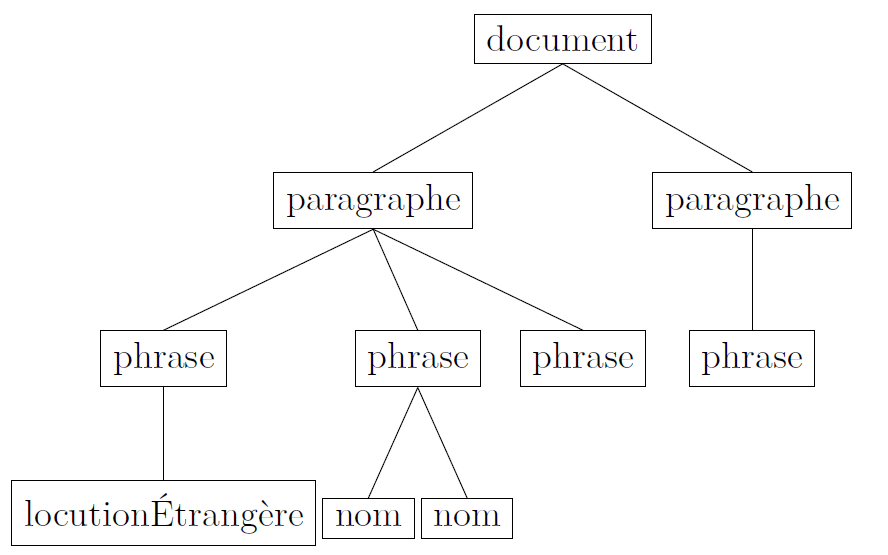
\includegraphics[width=\textwidth]{images/arbor1.png}
  
  \textit{Arborescence de l'exemple précédent}
\end{frame}

\begin{frame}
\frametitle{Arborescence plus précise}
    \noindent
  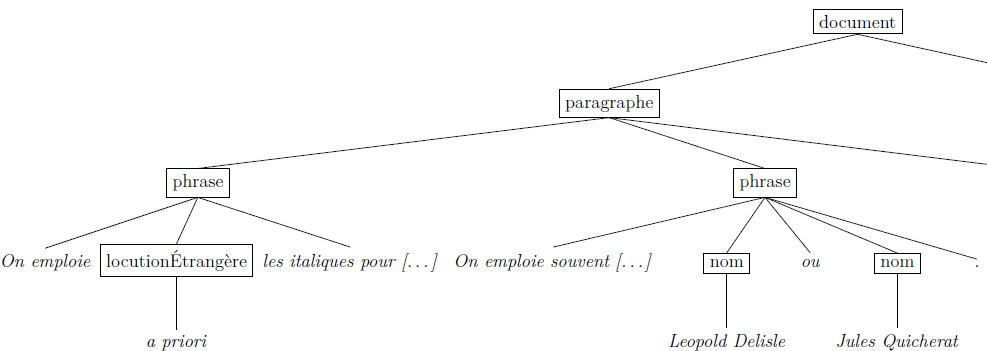
\includegraphics[width=\textwidth]{images/arbor2.png}
\end{frame}

\begin{frame}[fragile]

\frametitle{Puissance et limitation de XML}
\ttfamily\fontsize{8.5pt}{9pt}
\selectfont

\begin{exampleblock}{Bien formé}
	\noindent\ttfamily\mbox{}{\color{blue}<\textbf{auteur}>}\mbox{}\newline 
	{\color{blue}<\textbf{nom}>}Dupont{\color{blue}</\textbf{nom}>}\mbox{}\newline 
	{\color{blue}</\textbf{auteur}>}
\end{exampleblock}

\begin{exampleblock}{Pas bien formé}
\begin{minted}{xml}
<auteur><nom>Dupont</auteur></nom>
\end{minted}
\end{exampleblock}

%TODO: modifier cet exemple
\begin{exampleblock}{Toujours pas bien formé}
	\begin{minted}{xml}
<poème type="douteux">
  <vers>À la fin de ce vers, je dis : <locutionÉtrangère>Sic</vers>
  <vers> transit gloria mundi</locutionÉtrangère></vers>
</poème>
	\end{minted}
\end{exampleblock}

\end{frame}

\begin{frame}
\frametitle{Le modèle OHCO \cite{Renear1993}}

Une perspective d'analyse d'un texte peut être décomposée en une \alert{Ordered Hierarchy of Content Objects}.

\begin{description}
\item[\textit{Ordered}] car le texte à une direction (du début vers la fin);
\item[\textit{Hierarchy}] car les éléments ont entre eux une relation hiérarchique (un chapitre contient des paragraphes, qui contiennent des phrases…)
\item[\textit{Content Objects}] d'\textit{objets de contenu} quelconques, terme suffisamment vague pour englober un peu tout, selon l'analyse portée sur le texte.
\end{description} 

Plutôt \alert{hierarchies} que \textit{hierarchy}: une par approche ou analyse d'un texte.


\end{frame}


\begin{frame}
\frametitle{XML comme métalangage (\textit{eXtensible})}

XML est un métalangage, c'est-à-dire qu'il permet de définir différents langages (des applications) avec chacun leur grammaire propre (par exemple la \textit{Text Encoding Initiative} ou \textsc{tei}; l'\textit{Encoded Archival Description} ou \textsc{ead}; 
ou \textsc{xhtml}).

Contrairement à d'autres langages à balise, XML ne propose pas un jeu de balise prédéfini, mais un ensemble d'éléments et de règles sur ce que doit être un document bien formé ou un document valide, et la manière de créer et mettre en œuvre des langages.

\end{frame}

%\begin{frame}
%\frametitle{De nombreux dialectes, qui peuvent être combinés}\begin{itemize}
%	
%	\item TEI, pour l'édition électronique savante;
%	\item EAD pour la description archivistique, EAC-CPF pour les référentiels;
%	\item MEI pour l'édition de notations musicales;
%	\item XHTML, pour les pages Web;
%	\item DocBook, pour la documentation;
%	\item OpenDocument Format, pour des documents de traitement de texte;
%	\item MarcXML, MODS pour la description bibliographique;
%	\item RDF/XML pour le web sémantique;
%	\item SVG pour les images vectorielles;
%	\item MathML pour les formules mathématiques. 
%\end{itemize} 

%Pour une liste, un peu datée (2005) : \url{http://xml.coverpages.org/xmlApplications.html}
%\end{frame}

\subsection{Pourquoi opter pour une édition électronique?}

\begin{frame}{Pourquoi opter pour une édition électronique?}{Rappel de notre définition initiale}


\begin{block}{Édition électronique savante (Digital scholarly edition)} 
	Une édition qui utilise les possibilités de l'outil informatique pour proposer
	\begin{itemize}
		\item une \textbf{représentation critique ou enrichie sémantiquement} d'une source ✔ ;
		%{\fontspec{Times New Roman} \textcolor{green}{✔} };
		\item des fonctionnalités utiles à leur compréhension et leur analyse.
	\end{itemize}
\end{block}  

%\begin{block}{Édition électronique savante (Digital scholarly
%                                edition)} Une édition qui explicite la structure et le sémantisme d'un certain nombre de phénomènes propres au texte ou à la source pour en permettre le traitement par un ordinateur.  
%\end{block} 

\end{frame}

\begin{frame}
\frametitle{L'encodage sémantique et ses avantages}
\begin{itemize}	
	\item Rend le ``sémantisme implicite'' (ou, plutôt, l'interprétation, l'analyse critique) d'un document compréhensible par un ordinateur et l'explicite;
	\item Mise en forme indépendante du document, gérée à part et (re)configurable;
	\item Permet une exploitation utilisant le texte encodé comme base de données (fouille de données, \textit{information retrieval}, traitement automatique du langage, etc.) 
\end{itemize} 
\end{frame}

\begin{frame}
\frametitle{Les avantages techniques d'XML}
\begin{itemize}
\item Pérennité et interopérabilité, 
\item multiplicité des usages à partir d'un même document
	\begin{itemize}
	\item mise en forme;
	\item exploitation (recherche avancée, analyse quantitative, etc.);
	\item réutilisation;
	\end{itemize} 
\item contenu lisible par l'humain autant que par l'ordinateur;
%\item existence de nombreux dialectes et applications;
\item environnement de travail.
\end{itemize}
\end{frame}

\begin{frame}
\frametitle{XML comme format pivot}

    \noindent
  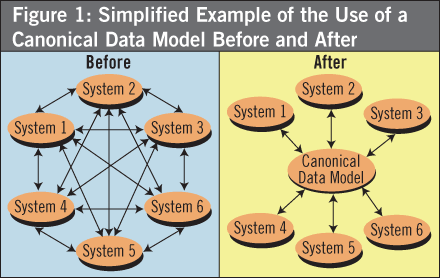
\includegraphics[width=0.8\textwidth]{images/formatPivot.jpg}
  
  {\footnotesize
  \textit{extr. de \textit{Steve Hoberman, « Canonical Data Model », \textit{Information Management Magazine}, en ligne : \url{http://www.information-management.com/issues/2007_50/10001733-1.html} (consulté le 14 nov. 2014)}.}}
\end{frame}

%\begin{frame}
%\frametitle{Une chaîne éditoriale qui prend appui sur la TEI}
%    \noindent
%  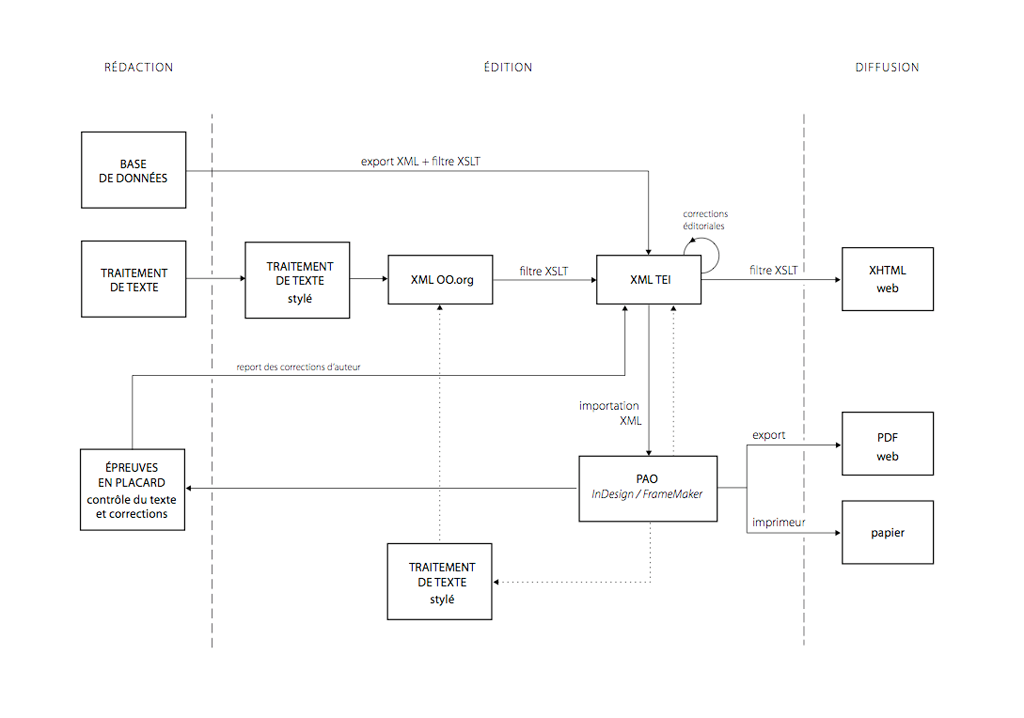
\includegraphics[width=0.8\textwidth]{images/chainePUCaen.jpg}
%  
%  {\footnotesize
%  \textit{La chaîne éditoriale des P.U. de Caen (\xref{http://scd.unicaen.fr/recherche/mrsh/document_numerique/projets/chaine_editoriale}{http://scd.unicaen.fr/recherche/mrsh/document\textunderscore numerique/projets/chaine\textunderscore editoriale}. Voir aussi la présentation de Pierre-Yves Buard, disponible en ligne, \xref{http://www.aedres.fr/pdf/XML-CR-19juin2009.pdf}{})}
%  }
%\end{frame}

\begin{frame}
\frametitle{Multiplicité des usages: ex. d'un chaîne éditoriale qui combine analyse et publication}
    \noindent
  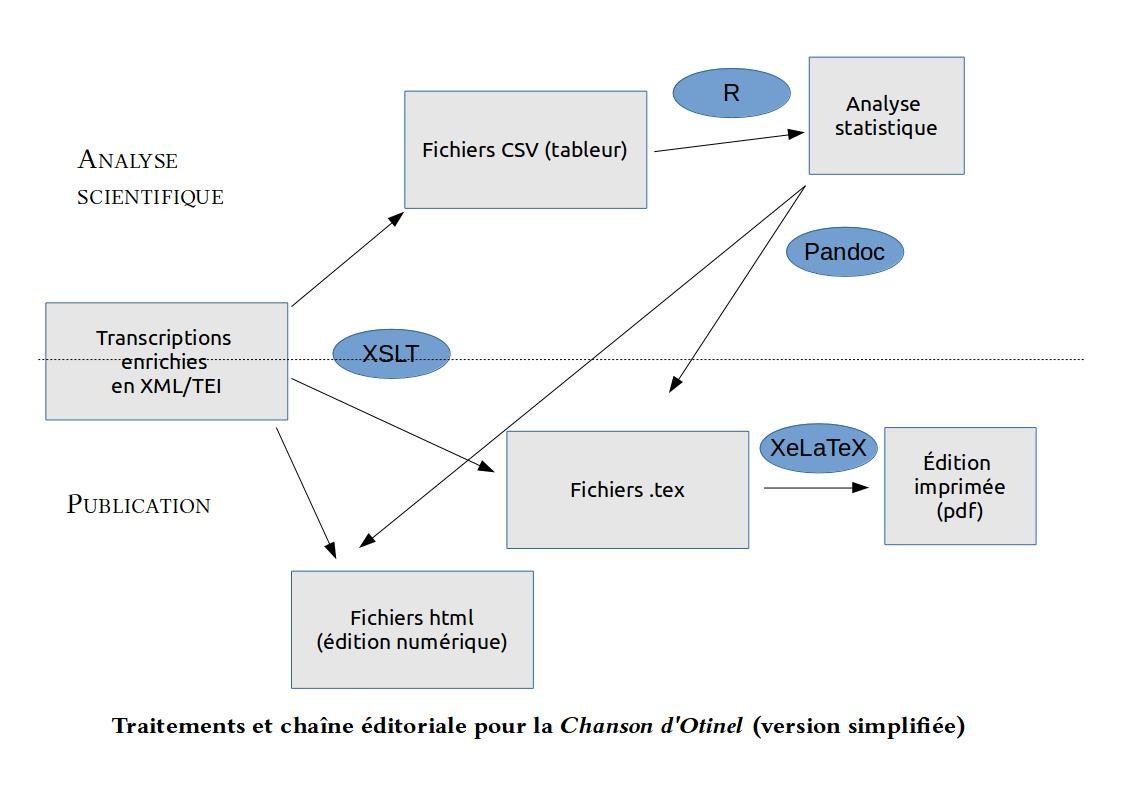
\includegraphics[width=\textwidth]{images/Chaine_editoriale.jpg}
\end{frame}

\begin{frame}{Publier sous différents formats}
	Convertir en xhtml pour une publication en ligne ou en \LaTeX{} pour une édition imprimée…
	
	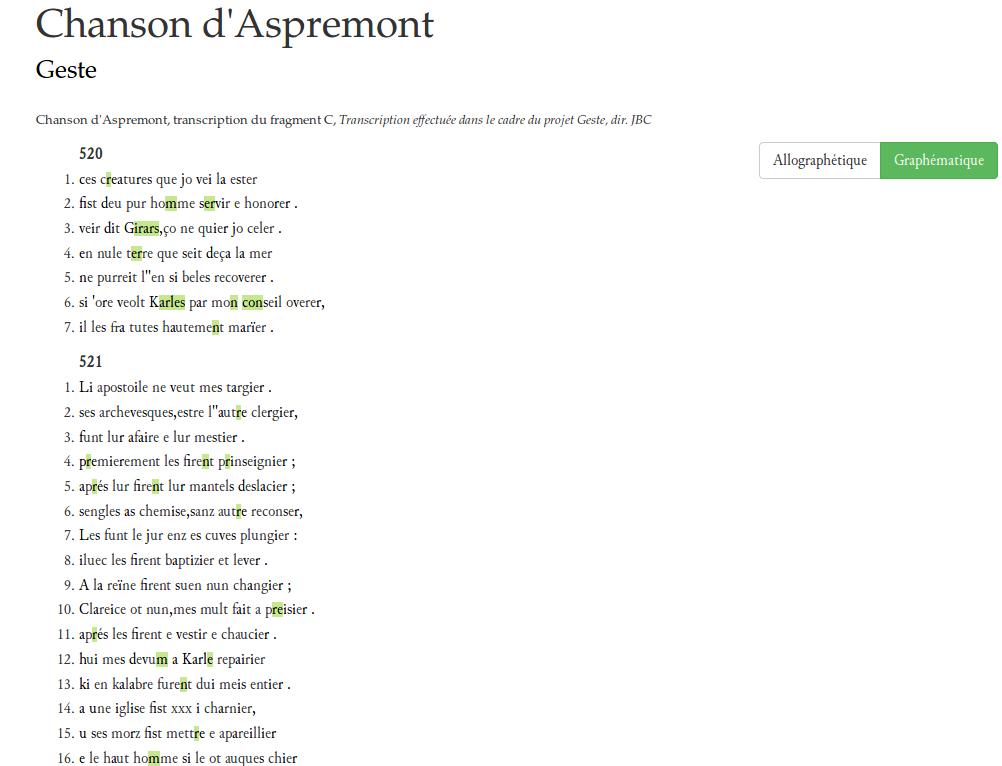
\includegraphics[width=0.45\textwidth]{images/Aspremont_Nemo.png}
	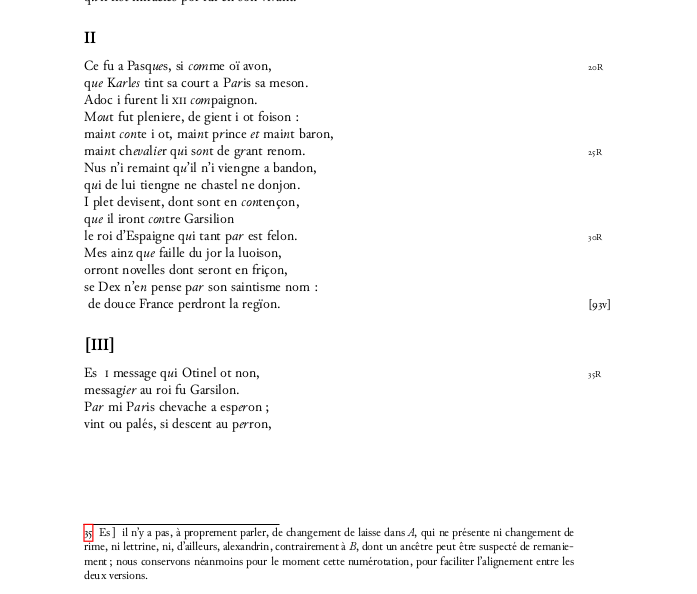
\includegraphics[width=0.45\textwidth]{images/Otinel_impr.png}
	
	Ex. de conversions \textsc{xml/tei} vers d'autres formats, \url{http://www.tei-c.org/oxgarage/}.
\end{frame}


\begin{frame}
\frametitle{Analyser ses données}
\begin{center}
  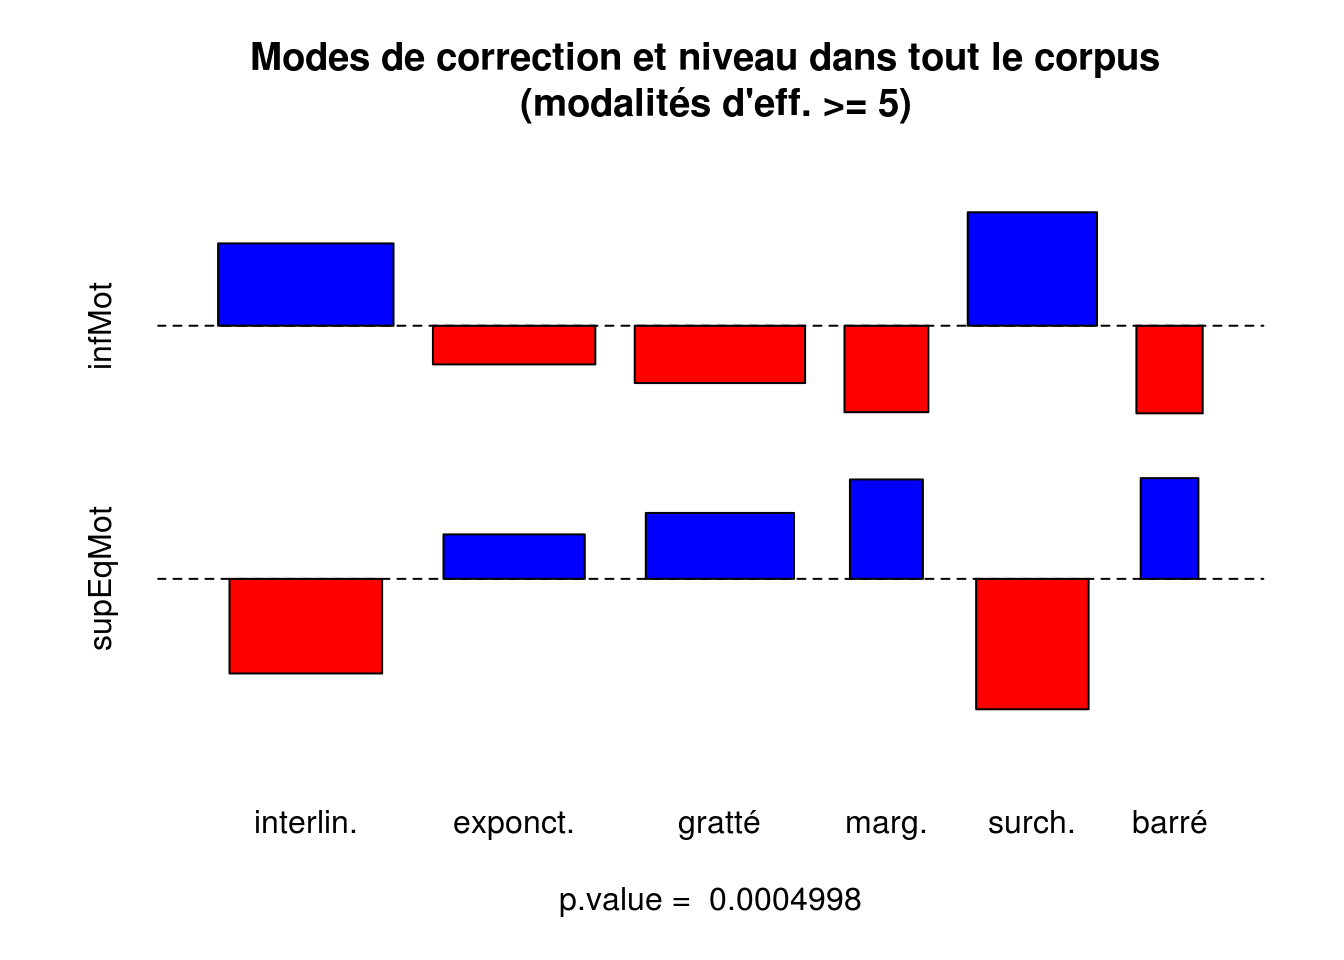
\includegraphics[width=0.75\textwidth]{images/global_corr_bc.png}
\end{center}
  { \footnotesize \textit{Modes de correction employés par les scribes et niveau de ces corrections} (ms. de la \textit{Chanson d'Otinel})}
\end{frame}

\begin{frame}
	\frametitle{Concevoir de nouvelles fonctionnalités}
	
	%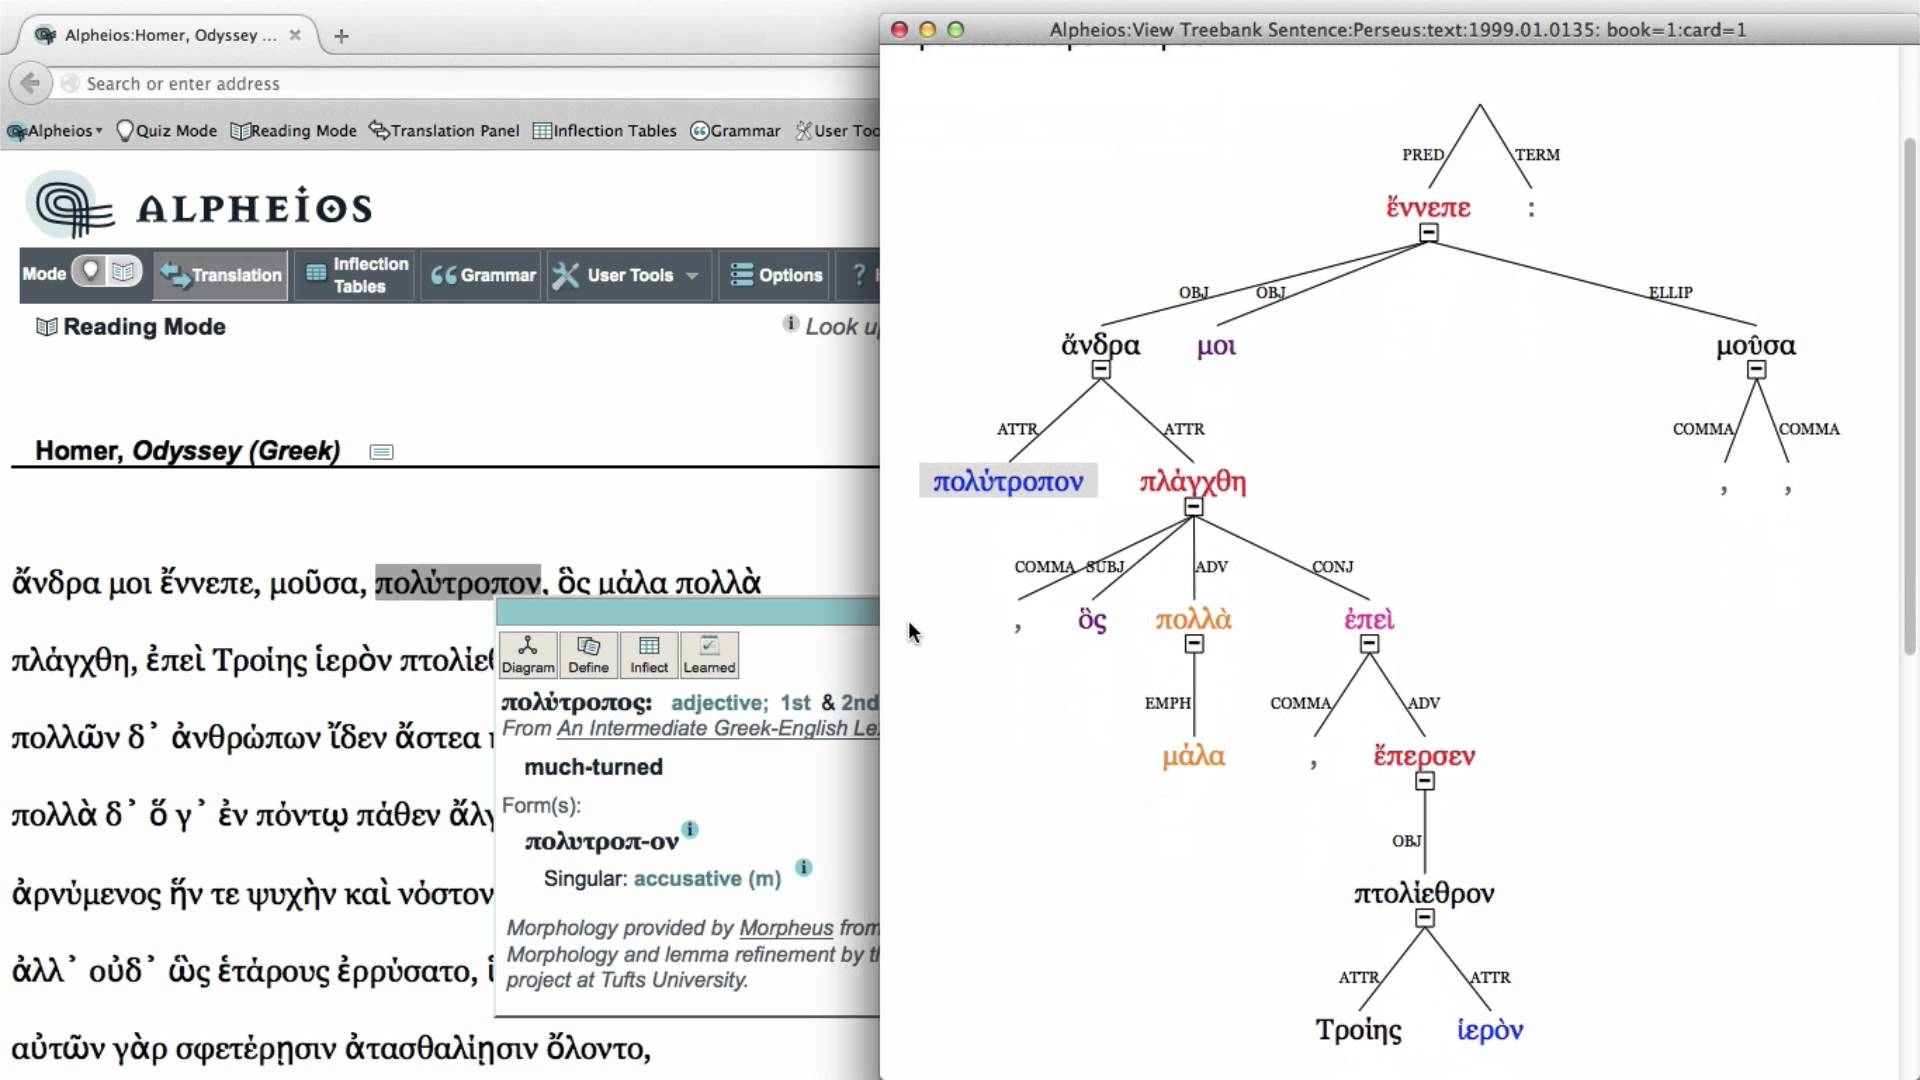
\includegraphics[width=\textwidth]{images/Alpheios_odyssee.jpg}
	
	\begin{columns}
	    \begin{column}{0.7\textwidth}
	        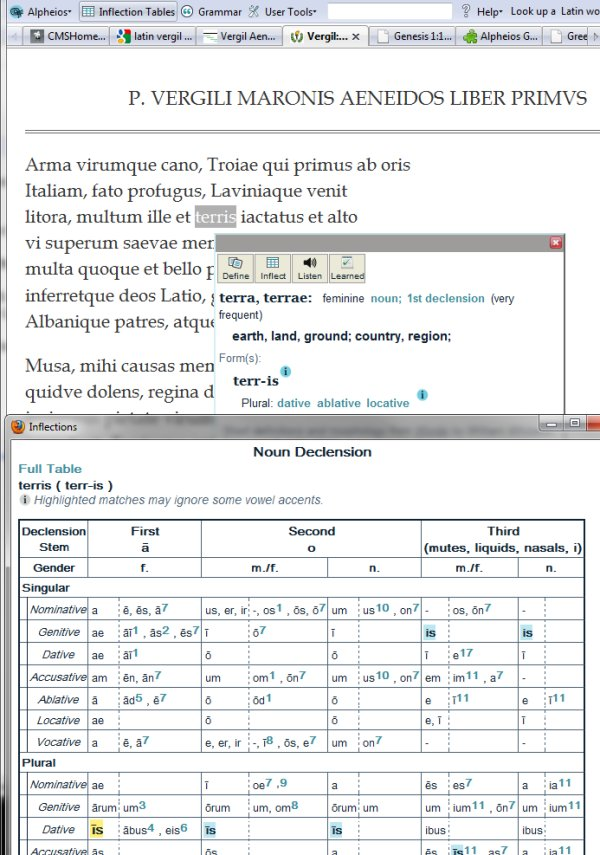
\includegraphics[height=0.9\textheight]{images/Alpheios_eneide.jpg}
	    \end{column}
	    \begin{column}{0.3\textwidth}
	        Afficher les \alert{paradigmes morphologiques}\\ ou \\ \alert{l'annotation syntaxique}
	    \end{column}
	    
	\end{columns}
	
\end{frame}

\begin{frame}
\frametitle{Nouvelles fonctionnalités -- annotation syntaxique}

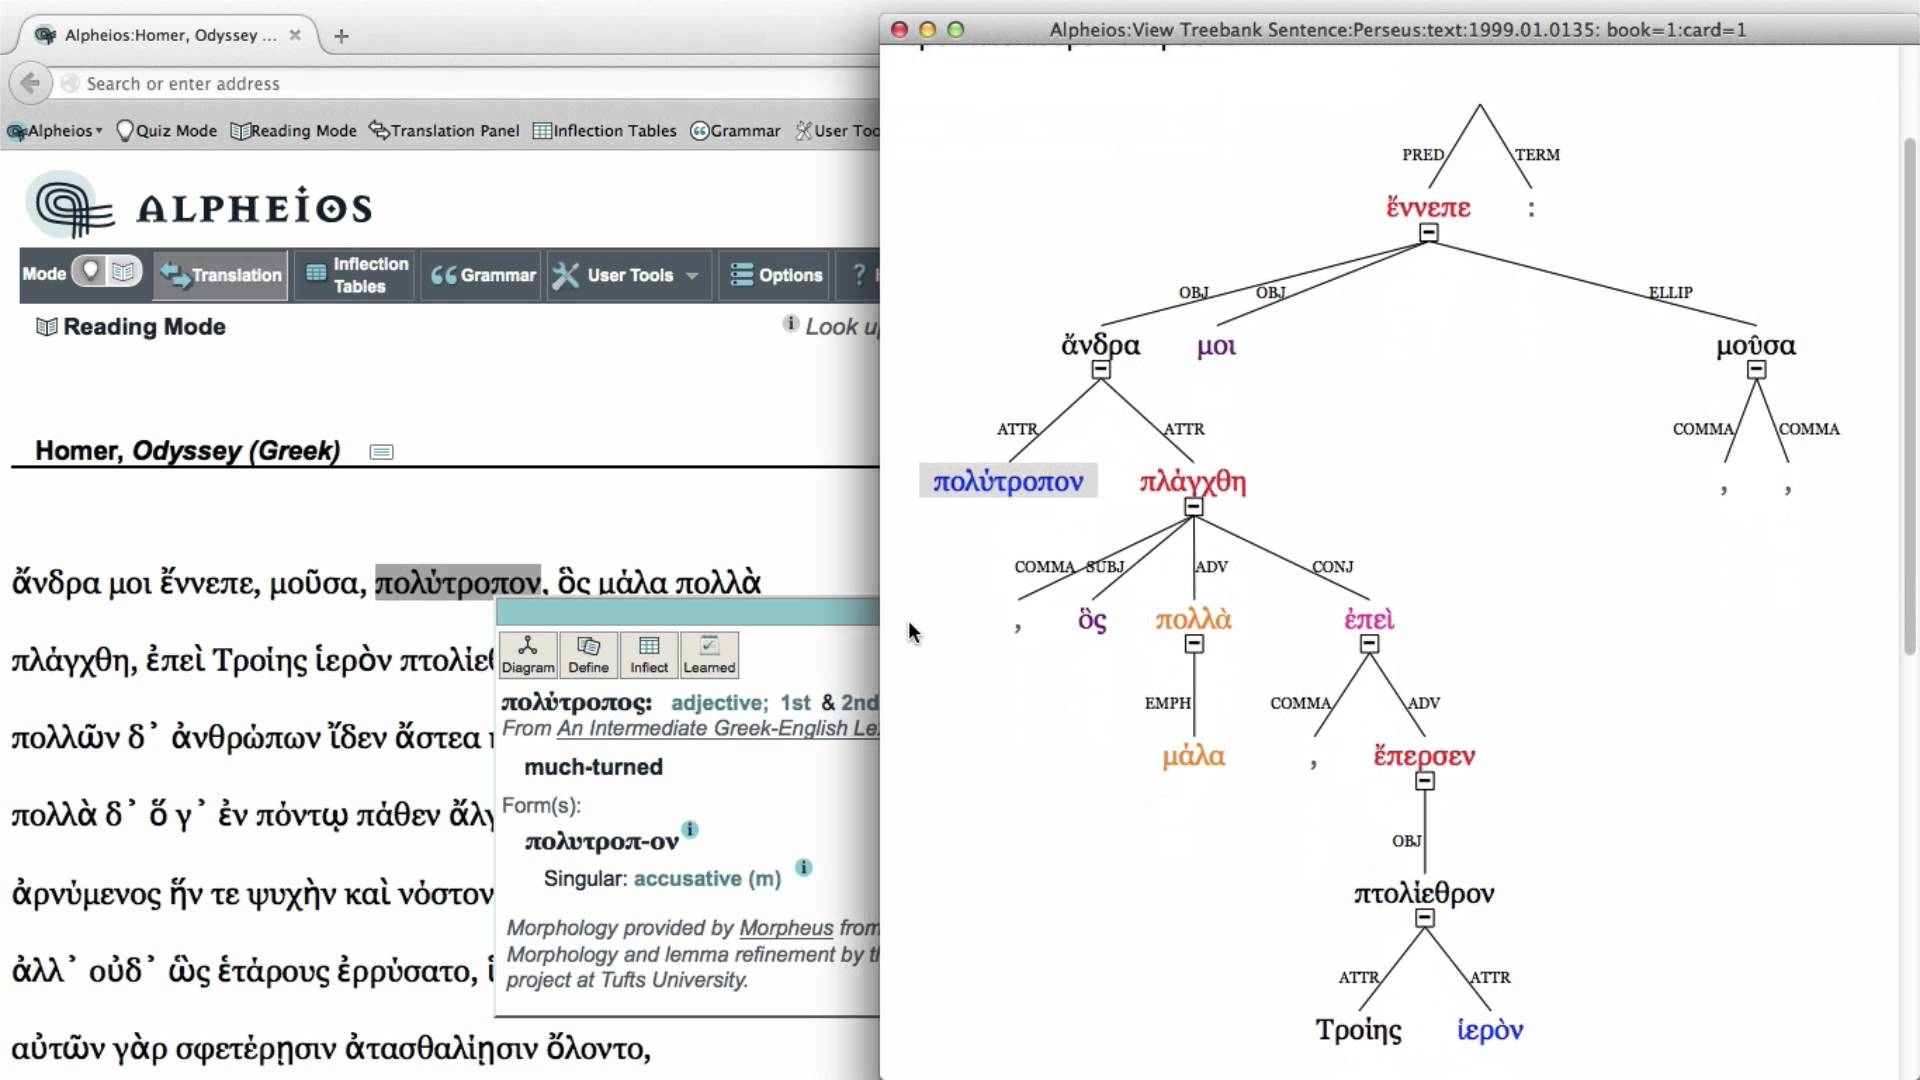
\includegraphics[width=\textwidth]{images/Alpheios_odyssee.jpg}
%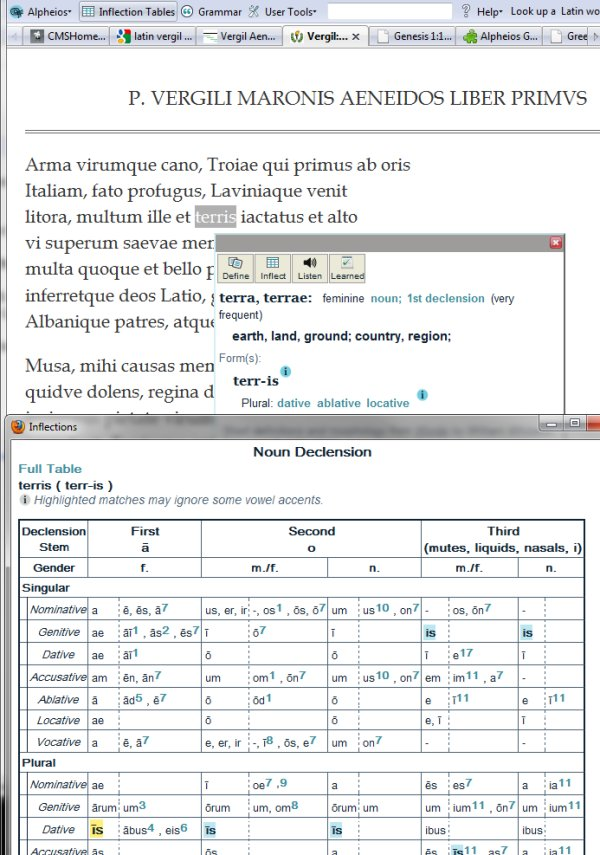
\includegraphics[height=\textheight]{images/Alpheios_eneide.jpg}

\end{frame}

%\subsection[Les langages à balise]{Les langages à balise: des premières expérimentations au XML et à la {\orgName Text Encoding Initiative}}
%
%\begin{frame}[fragile]
%\frametitle{Les langages à balise}{Des premières expérimentations au XML et à la {\orgName Text Encoding Initiative}}
%
%\ttfamily\fontsize{8.5pt}{9pt}\selectfont
%
%\begin{exampleblock}{COCOA (1965)}
%\begin{minted}{xml}
%<W SHAKESPEARE> <T HAMLET> <A 1> <S 1>
%\end{minted}
%\end{exampleblock}
%
%\ttfamily\fontsize{8.5pt}{9pt}\selectfont
%
%\begin{exampleblock}{SCRIPT et IBM’s Document Composition Facility Generalized Markup Language (GML, 1969)}
%	:h1 id=chap1. ceci est un titre de niveau 1, avec un attribut (id) chap1\\
%	:p. ceci est un paragraphe\\
%	:ul \\
%	:li. un item de liste \\
%	:li. et un second \\
%	:eul. \\
%	:xmp. des examples \\
%	:exmp. \\
%	:p. et d'autres balises encore 
%\end{exampleblock}
%\end{frame}
%
%\begin{frame}
%\frametitle{SGML (1986) et la naissance de XML (1996)}
%\noindent
%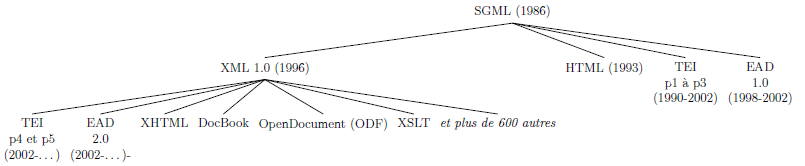
\includegraphics[width=\textwidth]{images/naissanceXML.png}
%\end{frame}
%
%\begin{frame}
%\frametitle{Les Principes de Poughkeepsie (1987)}
%
%Proposer des \textit{Guidelines} (recommandations) avec pour objectifs:
%
%\begin{itemize}
%\item[1] provide a standard format for data interchange in humanities research.
%\item[2] suggest principles for the encoding of texts in the same format.
%\item[3] define a recommended syntax for the format, a metalanguage for the description of text-encoding schemes, describe the new format and representative existing schemes both in that metalanguage and in prose ;
%\item[4] propose sets of coding conventions suited for various applications.
%\item[5] include a minimal set of conventions for encoding new texts in the format.
%\end{itemize} 
%\end{frame}
%
%\begin{frame}
%\frametitle{Les Principes de Poughkeepsie (1987)}
%
%\begin{itemize}\small
%\item[6] The guidelines are to be drafted by committees on text documentation, text representation, text interpretation and analysis, metalanguage definition and description of existing and proposed schemes, coordinated by a steering committee of representatives of the principal sponsoring organizations.
%\item[7] Compatibility with existing standards will be maintained as far as possible.
%\item[8] A number of large text archives have agreed in principle to support the guidelines in their function as an interchange format. We encourage funding agencies to support development of tools to facilitate this interchange.
%\item[9] Conversion of existing machine-readable texts to the new format involves the translation of their conventions into the syntax of the new format. No requirements will be made for the addition of information not already coded in the texts.
%\end{itemize} 
%\end{frame}
%
%
%\begin{frame}
%\frametitle{Repères chronologiques}\begin{itemize}
%
%\item 1987, établissement de la Text Encoding Initiative par trois sociétés savantes : Association for Computers and the Humanities, Association for Literary and Linguistic Computing et Association for Computational Linguistics
%\item 1990, TEI Proposal 1 (TEI P1), Guidelines for the Encoding and Interchange of Machine-Readable Texts, dir. Michael Sperberg-McQueen et Lou Burnard,
%\item 1992-1993, TEI P2, phase d'expansion
%\item 1994, TEI P3, considérée comme la première version complète
%\item 2000, naissance du TEI Consortium,
%\item 2001-2004, TEI P4 :> introduction du XML (à côté de SGML)
%\item 2007-..., TEI P5 (v.1.0) : abandon de SGML, autre phase d'accroissement ; mises à jour bi-annuelles ; 26 juillet 2013, v. 2.5 ; v. 2.7.0, 16 sept. 2014
%\end{itemize} 
%\end{frame}
%
%
%
%

\section[Outils et méthodes]{Outils et méthodes de l'édition électronique}

%\subsection[La Text Encoding Initiative et sa structure d'ensemble]{La {\orgName Text Encoding Initiative} et sa structure d'ensemble}
%
%\begin{frame}[fragile, shrink]
%\frametitle{La \textit{Text Encoding Initiative} et sa structure d'ensemble}
%
%\alert{Un modèle d'ensemble et de nombreuses applications }
%
%Les \textit{Guidelines}: \url{http://www.tei-c.org/release/doc/tei-p5-doc/en/html/}
%
%Distinguer,
%\begin{itemize}
%\item le modèle abstrait de données (ensemble des concepts et les relations entre ces concepts);
%\item les implémentations techniques du modèle (retranscription des contraintes formelles par le biais d'une grammaire XML)
%\end{itemize} 
%mais aussi
%\begin{itemize}
%\item le cadre général (le modèle des \textit{Guidelines} dans son ensemble)
%\item les implémentations particulières (répondre à des besoins spécifiques, liés à un outil, un projet, etc.), {\footnotesize par ex. \textit{EpiDoc} pour l'épigraphie, les modèles de l'\textsc{enc} pour les chartes et documents d'archives, le modèle de la \textit{Base de français médiéval}, etc.}
%\end{itemize} 
%
%\end{frame}
%
%\begin{frame}
%\frametitle{La Structure d'ensemble de la TEI: les modules}
%    \noindent
%  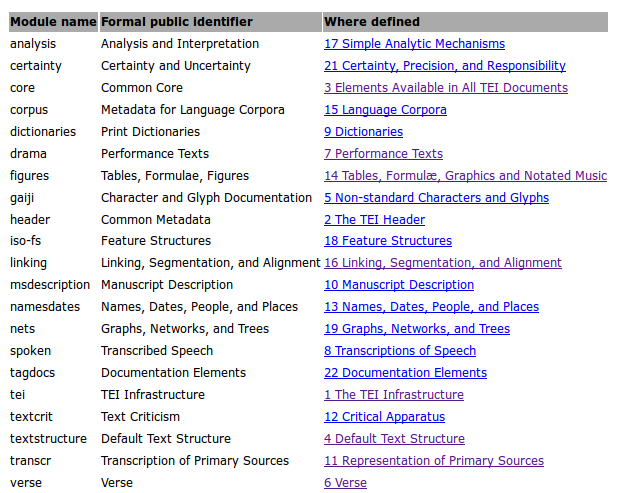
\includegraphics[width=0.9\textwidth]{images/modulesTEI.png}\textit{Les modules de la TEI}
%\end{frame}
%
%\begin{frame}
%\frametitle{Modules obligatoires (communs à tous les documents TEI)}\begin{itemize}
%
%\item \textsf{tei} : définition des classes, macros et types de données
%\item \textsf{textstructure} : éléments de base pour structurer un texte de type livre
%\item \textsf{core} : éléments disponibles dans tous les documents TEI
%\item \textsf{header} : en-tête TEI (métadonnées du document)
%\end{itemize} 
%\end{frame}
%
%\begin{frame}
%\frametitle{Module propres à un type d'objet, une approche, une discipline}\begin{itemize}
%
%\item \textsf{analysis} (analyse linguistique);
%\item \textsf{certainty} (niveaux de certitude et responsabilité) ;
%\item \textsf{corpus} (corpus) ;
%\item \textsf{drama} (textes d’art dramatique) ;
%\item \textsf{figures} (tableaux, figures et formules) ;
%\item \textsf{gaiji} (caractères non standard et glyphes) ;
%\item \textsf{iso-fs} (structures de traits) ;
%\item \textsf{linking} (liens, segmentation, alignements) ;
%\item \textsf{msdescription} (description des manuscrits) ;
%\item \textsf{namesdates} (noms, dates, lieux) ;
%\item \textsf{nets} (graphes, réseaux, arbres) ;
%\item \textsf{tagdocs} (documentation) ;
%\item \textsf{textcrit} (apparat critique) ;
%\item \textsf{transcr} (transcription des sources primaires) ;
%\item \textsf{verse} (vers).
%\end{itemize} 
%\end{frame}
%

\subsection[La modélisation comme outil d'analyse]{La modélisation comme outil d'analyse: construire son propre modèle TEI}

\begin{frame}[fragile]
\frametitle{La modélisation comme outil d'analyse: construire son propre modèle TEI}{}

\begin{block}{Modélisation} Opération par laquelle on établit le modèle d'un système complexe, afin d'étudier plus commodément et de mesurer les effets sur ce système des variations de tel ou tel de ses éléments composants » \end{block} { \small\textit{(J. Giraud, P. Pamart, J. Riverain, Les nouveaux mots \og{}dans le vent\fg{}, Paris, France, 1974).} }

\medskip

Définir un modèle adapté:
\begin{itemize}
\item aux documents que l'on édite;
\item à la perspective scientifique dans laquelle l'édition est réalisée;
\item aux moyens (temps, financement, …) dont on dispose.
\end{itemize}

\end{frame}


%\subsubsection{Édition d'un imprimé ancien: structure physique et logique (et niveau de granularité)}

\begin{frame}[fragile]
\frametitle{Édition d'un imprimé ancien: structure physique et logique (et niveau de granularité)}
\begin{itemize}
\item représentation de la structure physique de la source (feuillets, pages, lignes, etc.);
\item représentation de la structure logique (parties, chapitres, etc.);
\end{itemize}

\begin{block}{Granularité}
 degré de finesse ou précision d'un modèle, conçu comme le niveau de son plus petit composant. Plus la granularité est grande, plus on descend dans la modélisation (niveau phrase, mot, graphème, etc.) --~et plus on ajoute de balises.
\end{block}


\end{frame}
%
%\begin{frame}[fragile]
%\frametitle{Artamène ou le Grand Cyrus}
%{\footnotesize Madeleine et Georges de Scudéry, \textit{Artamène ou le Grand Cyrus}, \url{http://www.artamene.org/}, encodé en utilisant la TEI Lite}
%        \bgroup\ttfamily\fontsize{7pt}{8pt}
%        \selectfont
%\begin{minted}{xml}
%<body>
%    <div0 type="partie" id="page_CYRUS01" n="I">
%        <head type="epitre"
%            n="Epitre dédicatoire à Mme la Duchesse de Longueville placée en tête du 1er volume">
%            <pb id="page_epitre_dedicatoire_volume1_1" n="V01-I001"
%            /> A MADAME <lb/>LA DUCHESSE <lb/>DE LONGUEVILLE.
%            <!--[...]-->
%        </head>
%        <div1 id="page_CYRUS0101" type="livre" n="premier">
%            <div2 id="page_CYRUS010101" type="sequence"
%                n="Incendie de Sinope">
%                <p>
%                    <pb id="page_1" n="V01-P005"/>L'embrazement de la
%                    Ville de Sinope estoit si grand, que tout le Ciel
%                    ; toute la Mer ; <!-- [...] -->
%                    <pb id="page_2" n="V01-P006"/>vers la plus grande
%                    partie de la Ville, qu'elles avoient desja toute
%                    embrazée ; et de laquelle elles n'avoient
%                    <!-- [...] -->
%                </p>
%            </div2>
%        </div1>
%    </div0>
%</body>
%\end{minted}
%        
%\egroup
%    
%\end{frame}
%
%\begin{frame}[fragile]
%\frametitle{Champ Fleury}
%{\footnotesize
%\textit{Champ Fleury}, dans la BVH, \url{http://www.bvh.univ-tours.fr:8080/xtf/view?docId=tei/B410186201\textunderscore I65/B410186201\textunderscore I65\textunderscore tei.xml}}
%
%\bgroup\ttfamily\fontsize{7pt}{8pt}
%        \selectfont
%\begin{minted}{xml}
%<docImprint>
%    <lb/>Ce Livre est Privilegie pour Dix Ans <lb/>Par Le Roy nostre
%    Sire. &amp; est a ven- <lb rend="hyphen"/>dre a
%    <pubPlace>Paris</pubPlace> sus <placeName type="rue">Petit
%        Pont</placeName> a l’Enseigne <lb/>du <placeName
%            type="enseigne">Pot Casse</placeName> par <publisher>Maistre <name>
%                <choice>
%                    <orig>Geofroy</orig>
%                    <reg>Geoffroy</reg>
%                </choice>
%                <lb/>Tory</name>
%            </publisher> de <placeName type="ville">Bourges</placeName> /
%    Libraire, &amp; Au- <lb rend="hyphen"/>theur du dict Livre. Et
%    par <publisher>
%        <name>Giles Gour- <lb rend="hyphen"/>mont</name>
%    </publisher> aussi Libraire demourant en la <lb/>
%    <placeName type="rue">Rue <name>sainct Jaques</name>
%    </placeName> a l’Enseigne des <lb/>
%    <placeName type="enseigne">Trois Coronnes</placeName>. </docImprint>
%<lb/>
%<imprimatur rend="center">
%    <lb/>
%    <lb/>PRIVILEGIE POUR DIX ANS.</imprimatur>
%\end{minted}
%
%\egroup
%    
%\end{frame}
%
%%\subsubsection{Éditions de documents d'archives et encodage des parties du discours diplomatique}
%
%\begin{frame}[fragile]
%\frametitle{Éditions de documents d'archives et encodage des parties du discours diplomatique}{}
%\end{frame}
%
%\begin{frame}[fragile]
%\frametitle{Le cartulaire blanc de Saint-Denis : chapitre de Beaurain}
%{\tiny acte n\textsuperscript{o} 2, en ligne: \url{http://saint-denis.enc.sorbonne.fr/cartulaire/tome1/beaurain/acte2}}
%
%\bgroup\ttfamily\fontsize{7pt}{8pt}\selectfont
%\begin{minted}{xml}
%<div type="transcription" xml:lang="lat">
%    <p>Antiquorum docemur exemplis ut querelas [...]. Quapropter ego
%        <expan>W<ex>illelmus</ex></expan>, [...] qualiter
%        super multis querelis que inter nos et nobilem virum
%        <expan>G<ex>uidonem</ex></expan> de Caprosia diutius
%        agitate fuerant, mediantibus viris prudentibus [...] 
%        presenti pagina notum facimus quod
%        prenominatus <expan>G<ex>uido</ex></expan> quatuor nemora,
%        videlicet <foreign xml:lang="fro">Sorforest </foreign> et
%        <foreign xml:lang="fro">Gaini</foreign> et Bellam Pennam
%        et Hayam de Ambesiis<ref type="note" n="3"
%            target="#beaurain-acte2-n-3"/> [...] excepta quoque
%        chathena<ref type="note" n="4"
%            target="#beaurain-acte2-n-4"/> una [...] de 
%        <app n="e">
%          <lem wit="#beaurain-acte2-B">Dampni<supplied
%                    source="#beaurain-acte2-indiqué-i-noir"
%                    >pe</supplied>tra</lem>
%          <note xml:lang="fre"><foreign xml:lang="lat"
%            >pe</foreign> largement effacé dans B, rétabli
%             d’après l’Anc. inv. noir</note>
%            </app>
%        quem emerat a Lamberto [...] </p>
%</div>
%\end{minted}
%\egroup
%    
%\end{frame}
%
%\begin{frame}[fragile]
%\frametitle{Le formulaire d'Odart Morchesne}
%{\tiny En ligne: \url{http://elec.enc.sorbonne.fr/morchesne/}}
%
%\bgroup\ttfamily\fontsize{7pt}{8pt}\selectfont
%\begin{minted}{xml}
%<text xml:id="morchesne_1-1" n="1.1" type="formule" subtype="article">
%    <front>
%        <head>Grace a plaidier par procureur</head>
%        <index><term type="auth_type" key="act_souv"/></index>
%    </front>
%    <body>
%        <div type="transcription" xml:lang="fro">
%            <p><seg function="intitulatio">Charles, par la grace
%                de Dieu roy de France,</seg>
%                <seg function="address">a tous ceulz qui ces
%                    presentes lettres verront,</seg>
%                <seg function="salutatio">salut.</seg>
%                <seg function="notification">Savoir faisons</seg>
%                <seg function="dispositio">nous de grace especial
%                    <seg function="verb">avoir octroyé</seg>
%                    <seg function="beneficiary">a nostre amé et feal
%                        clerc, notaire et secretaire maistre Odart
%                        Morchesne, prieur de l'eglise collegial de Saint
%                        Aignen en Berry et penancier d'Orleans</seg>,
%                    <note> L'église collégiale, siège de la paroisse
%                        de Saint-Aignan (Loir-et-Cher, ch.-l. cant.), fut
%                        fondée, comme le laissent supposer des indices
%                        archéologiques, vers le milieu du XIe siècle […]
%                        (<bibl><title>Pouillés de la
%                            province de Bourges</title>, t. I, p. 139</bibl>), […]
%                    </note>
%                    <seg function="donatio">que il tant cause de ses
%                        benefices comme autrement en toutes ses causes et
%                        quereles meues et a mouvoir contre tous ses
%                        adversaires par devant tous juges seculiers de
%                        nostre royaume, en demandant et en defendant, soit
%                        receu par procureur en parlement et dehors jusques
%                        a un an.</seg></seg>
%                <seg function="dating">Donné a Bourges le XXV<hi
%                    rend="sup">e</hi> jour de juing, l'an de grace mil
%                    quatre cens vint et cinq, et de nostre regne le
%                    tiers.</seg>
%            </p>
%        </div>
%    </body>
%</text>
%\end{minted}
%        
%\egroup
%    
%\end{frame}

\begin{frame}
\frametitle{Le développement de modèles spécifiques}
\alert{Les actes diplomatiques édités par l'École des chartes}

Voir le modèle développé à l'École pour l'édition d'un acte en TEI : \url{http://developpements.enc.sorbonne.fr/diple/schema/acte}

Exemple de la définition de l'élément \texttt{<seg>}, de son attribut \emph{@function}, et de son jeu de valeur défini (localement), ‘invocation’, ‘intitulatio’, ‘salutatio’, etc. (qui renvoient à la version en ligne du Vocabulaire international de la diplomatique); \url{http://developpements.enc.sorbonne.fr/diple/schema/acte\#def\textunderscore diplomatique}
\end{frame}

%\begin{frame}
%\frametitle{Les \textit{Anglo-Saxon charters}}
%{\tiny en ligne: \url{http://www.aschart.kcl.ac.uk/diplomatic/idx\textunderscore invocation.html}}
%
%    \noindent
%  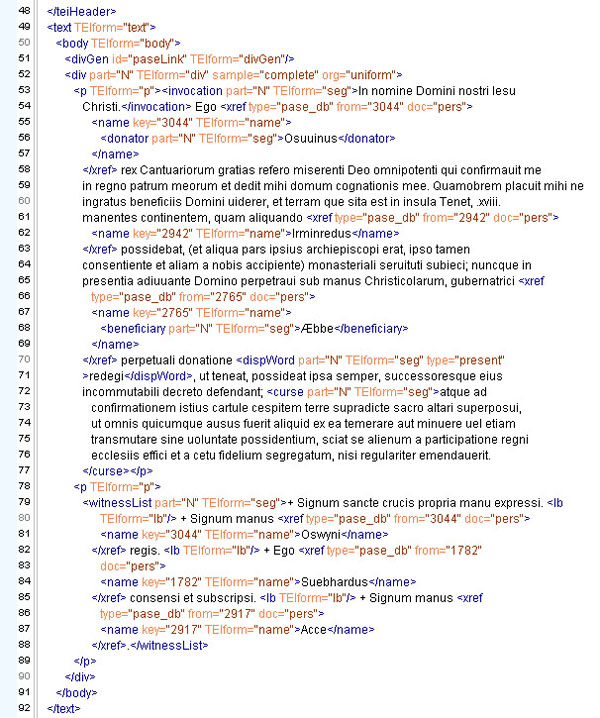
\includegraphics[width=\textwidth]{images/ASCharters_xml_sample.jpg}
%  
%  \textit{Extrait de code donné dans l'introduction technique}
%\end{frame}

%\subsubsection{Modéliser les interventions éditoriales}
%
%\begin{frame}[fragile]
%\frametitle{Modéliser les interventions éditoriales}{Corrections, régularisations, normalisations, sur le plan sémantique, linguistique, (paléo)graphique}
%\end{frame}
%
%\begin{frame}
%\frametitle{L'édition à visée linguistique d'une lettre contemporaine (facsimile)}
%    \noindent
%  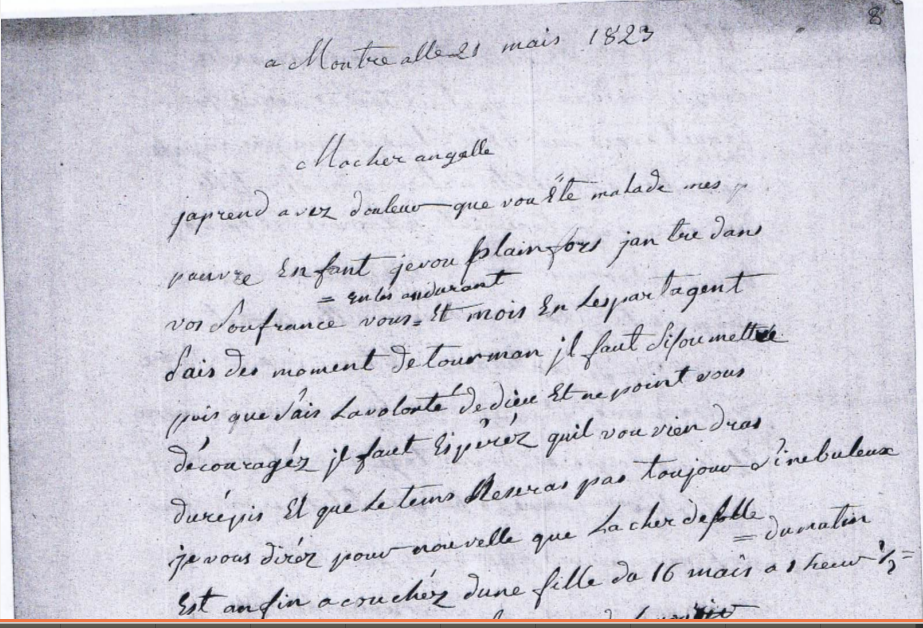
\includegraphics[width=\textwidth]{images/CherrierLettre.png}
%\end{frame}
%
%\begin{frame}[fragile]
%\frametitle{L'édition à visée linguistique d'une lettre contemporaine (encodage du corps de la lettre)}
%        \bgroup\ttfamily\fontsize{7pt}{8pt}\selectfont
%\begin{minted}{xml}
%<div type="letter"><pb n="1"/><lb/>
%<opener>
%    <dateline>
%        <choice><orig>a</orig><reg>À</reg></choice>
%        <name type="place" ref="Montréal"
%            ><w><choice><orig>Montre<space/>al</orig><reg>Montréal</reg></choice></w>
%        </name>
%        <w>le</w>
%        <date when="1823-05-21">21 
%            <choice><orig>mais</orig><reg>mai</reg></choice>
%            1823</date>
%    </dateline>
%    <salute><lb/>Ma
%        <choice><orig>cher</orig><reg>chère</reg></choice>
%        <name type="person" ref="#A_Cornud"><choice>
%            <orig>angelle</orig>
%            <reg>Angelle</reg>
%        </choice></name><pc type="supplied">,</pc>
%    </salute>
%</opener>
%<p>
%    <lb/><w rend="elision"
%        ><choice><orig>j</orig><reg>J</reg></choice></w>
%    <w><choice><orig>aprend</orig><reg>apprends</reg></choice></w>
%    <choice><orig>avez</orig><reg>avec</reg></choice> douleur
%    que <choice><orig>vou</orig><reg>vous</reg></choice>
%    <choice><orig>Éte</orig><reg>êtes</reg></choice>
%    <choice><orig>malade</orig><reg>malades</reg></choice><pc
%        type="supplied">.</pc>
%    <choice><orig>mes</orig><reg>Mes</reg></choice>
%    <lb/><choice><orig>pauvre</orig><reg>pauvres</reg></choice>
%    <choice><orig>Enfant</orig><reg>enfants</reg></choice><pc
%        type="supplied">,</pc> je
%    <choice><orig>vou</orig><reg>vous</reg></choice>
%    <choice><orig>plain</orig><reg>plains</reg></choice>
%    <!-- ... -->
%</p>
%</div>
%\end{minted}
%        
%\egroup
%    
%\end{frame}

%\begin{frame}[fragile]
%\frametitle{L'édition à orientation linguistique et paléographique d'un manuscrit médiéval}
%{\tiny La \textit{Queste del Saint Graal}, éd. Christiane Marchello-Nizia et A. Lavrentiev, \href{http://portal.textometrie.org/txm/texte/quete}{\texttt{http://portal.texto\-metrie.org/txm/texte/quete}}}
%
%\bgroup\ttfamily\fontsize{7.5pt}{8pt}\selectfont
%\begin{minted}{xml}
%<p n="1"><lb n="1"/><s n="1" xml:id="s_fro_1">
%    <supplied resp="#cmn" source="#ms_Z" reason="arraché">
%        <w type="PRE" xml:id="w106_000001">
%            <choice>
%                <me:norm>A</me:norm>
%                <me:dipl><hi rend="initiale">A</hi></me:dipl>
%                <me:facs><bfm:lettrine size="15" sizeAct="15"
%                    color="black" decoration="miniature"
%                    >A</bfm:lettrine></me:facs>
%            </choice>
%        </w>
%        <w type="DETdef" xml:id="w106_000002">
%            <choice>
%                <me:norm>la</me:norm>
%                <me:dipl>la</me:dipl>
%                <me:facs>la</me:facs>
%            </choice>
%        </w>
%        <w type="NOMcom" xml:id="w106_000003">
%            <choice>
%                <me:norm>veille</me:norm>
%                <me:dipl>ueille</me:dipl>
%                <me:facs>ueille</me:facs>
%            </choice>
%        </w>
%        <w type="PRE" rend="aggl" xml:id="w106_000004">
%            <choice>
%                <me:norm>de</me:norm>
%                <me:dipl>de</me:dipl>
%                <me:facs>de</me:facs>
%            </choice>
%        </w>
%        <w type="DETdef" rend="aggl" xml:id="w106_000005">
%            <choice>
%                <me:norm>la</me:norm>
%                <me:dipl>la</me:dipl>
%                <me:facs>la</me:facs>
%            </choice>
%        </w>
%    </supplied>
%</s>
%</p>
%\end{minted}        
%\egroup
%    
%\end{frame}
%
%\begin{frame}[fragile]
%\frametitle{Transcription d'un témoin de la \textit{Chanson d'Otinel}}
%        \bgroup\ttfamily\fontsize{7pt}{8pt}\selectfont
%\begin{minted}{xml}
%<lb/><l n="3" xml:id="M_l_3">
%  <gap reason="damage"/>
%  <unclear reason="damage"
%  ><w xml:id="M_w_000012"
%    >pt<choice><reg>i</reg><orig>ı</orig></choice>ze</w></unclear>
%  <gap reason="damage"/>
%  <w xml:id="M_w_000013"
%  ><choice><reg>a</reg><orig>ɑ</orig></choice>
%  <choice><reg>v</reg><orig>u</orig></choice>ez</w>
%  <w xml:id="M_w_000014"
%  ><choice><expan>v<ex>ost</ex>re</expan><abbr>urẽ</abbr></choice></w>
%  <w xml:id="M_w_000015"
%  >le<choice
%  ><reg>i</reg><orig>ı</orig></choice></w>
%  <w xml:id="M_w_000016"
%  >gerp<choice><reg>i</reg><orig>ı</orig></choice><orig>́</orig>e</w>
%</l>
%\end{minted}
%        
%\egroup
%    
%\end{frame}
%
%\begin{frame}[fragile]
%\frametitle{Une édition à visée paléographique, mettant en rapport texte et image}
%{\tiny \textit{Thélème}, Dossier no 88: 1109, septembre. Acte épiscopal (Sens), \url{http://theleme.enc.sorbonne.fr/dossiers/notice88.php}}
%        \bgroup\ttfamily\fontsize{7pt}{8pt}\selectfont
%\begin{minted}{xml}
%<div type="facsimile" rend="fax.jpg">
%    <div type="remarque">
%        <p>Note sur la transcription. Les “e cédillés” sont rendus
%            selon le cas par “æ” ou "œ".</p>
%    </div>
%    <div>
%        <p>
%            <seg rend="22,73,58,72,50,366,23,367" n="poly">
%                <expan>Chrismon</expan>
%            </seg>
%            <seg rend="64,70,520,61,520,95,63,102" n="poly">In
%                nomine D<expan>omi</expan>ni. DAIMBERTUS
%                archiep<expan>iscopu</expan>s.</seg>
%            <seg rend="55,107,571,95,574,127,55,136" n="poly"
%                >Notu<expan>m</expan> esse volum<expan>us</expan>
%                om<expan>n</expan>ib<expan>us</expan>
%                Chr<expan>ist</expan>i fidelib<expan>us</expan>
%                q<expan>u</expan>ia, cu<expan>m</expan> in
%                gremio</seg>
%            <seg rend="56,141,581,132,581,157,309,160,60,167"
%                n="poly">s<expan>an</expan>c<expan>t</expan>æ Matris
%                aeccl<expan>esi</expan>æ sacru<expan>m</expan>
%                cælebrarem<expan>us</expan>
%                c<expan>on</expan>ventu<expan>m</expan>, venit
%                in</seg>
%            <seg
%                rend="59,174,309,166,579,163,576,192,303,194,65,199"
%                n="poly">p<expan>re</expan>sentia<expan>m</expan>
%                n<expan>ost</expan>ram abbas
%                S<expan>an</expan>c<expan>t</expan>i Germani de
%                Prato Parisiensis</seg>
%            <!--...-->
%        </p>
%    </div>
%</div>
%\end{minted}
%        
%\egroup
%    
%\end{frame}

%\subsubsection{Modéliser la variance textuelle}
%
%\begin{frame}[fragile]
%\frametitle{Modéliser la variance textuelle}
%
%\alert{Des traditions médiévales aux brouillons d'écrivain}
%
%\end{frame}
%
%\begin{frame}[fragile]
%\frametitle{Une note d'apparat critique: le vers 3500 du \textit{Chevalier au lion}}
%
%{\tiny Pour le vers ‘Et s'espee qui fu coulans’ (\textit{éd. Hult, v. 3494}).}
%
%\bgroup\ttfamily\fontsize{8.5pt}{9pt}\selectfont
%\begin{minted}{xml}
%Et <app
%    type="synonymism">
%    <rdg wit="#H #P #V #F #A #S #R #M">s</rdg>
%    <rdg wit="#G" cause="paleographicConfusion">l</rdg>
%</app>'espee qui <app type="flectional">
%    <rdg>
%        <app type="graphic">
%            <rdg wit="#P #V #F #G #A #S #R">fu</rdg>
%            <rdg wit="#M">fut</rdg>
%        </app>
%    </rdg>
%    <rdg wit="#H">ert</rdg>
%</app>
%<app type="graphic">
%    <rdg wit="#H">colanz</rdg>
%    <rdg wit="#F">colans</rdg>
%    <rdg wit="#P #A #S #R">coulans</rdg>
%    <rdg wit="#V #G #M">coulanz</rdg>
%</app>
%\end{minted} 
%\egroup
%
%\end{frame}
%
%\begin{frame}[fragile]
%\frametitle{Une édition génétique de brouillon d'auteur}
%
%{\tiny Un brouillon de Stendhal (\textit{Des Périls de la Langue Italienne}), publié par \textit{Les manuscrits de Stendhal}, en ligne: \url{http://stendhal.msh-alpes.fr/}.}
%
%\bgroup\ttfamily\fontsize{7pt}{8pt}\selectfont
%\begin{minted}{xml}
%<surface><note place="margin" rend="Position_verticale : bas Position_horizontale : centre ">
%    <handShift scribe="Stendhal"/>
%    <p rend="Alignement : droite ">
%        <lb rend="Alignement : droite "/>exprimer
%        <lb rend="Alignement : droite "/>et non 
%        <lb rend="Alignement : droite "/>imprimer 
%        <lb rend="Alignement : droite "/>in the first phrase of the 
%        <lb rend="Alignement : droite "/>translation. 
%    </p>
%    <handShift scribe="Stendhal"/></note>
%    <note place="margin" rend="Position_verticale : milieu Position_horizontale : gauche ">
%        <handShift scribe="Colomb"/><p><lb/>Composition au sujet
%            <lb/>d'un écrit publié par
%            <lb/>Monti.
%        </p><handShift scribe="Stendhal"/></note>
%</surface>
%\end{minted}
%
%\egroup
%    
%\end{frame}
%
%%\subsubsection{Tableau de la tradition et notices de manuscrits}
%
%\begin{frame}[fragile]
%\frametitle{Tableau de la tradition et notices de manuscrits}
%\end{frame}
%
%\begin{frame}[fragile]
%\frametitle{Tableau de la tradition (Cartulaire blanc)}
%
%\bgroup\ttfamily\fontsize{7pt}{8pt}\selectfont
%\begin{minted}{xml}
%<div type="tradition">
%    <listWit>
%        <listWit xml:id="beaurain-acte1-copies">
%            <witness xml:id="beaurain-acte1-B"><label>B</label>. 
%                Cart. blanc, t. I, p. 537a-538a, n° I, précédé du
%                titre du chapitre, <quote xml:lang="lat"
%                    type="rubric">De Bello Ramo</quote>, et avec
%                reproduction du monogramme (p. 537b). </witness>
%            <witness xml:id="beaurain-acte1-C"
%                ><label>C</label>. Cart. Beaurain, p. 1-2.
%            </witness>
%        </listWit>
%        <listWit xml:id="beaurain-acte1-indiqué">
%            <head>Indiqué</head>
%            <witness xml:id="beaurain-acte1-indiqué-i-noir">Anc.
%                inv. noir, p. 157a, n° I : <quote type="summary"
%                    xml:lang="lat">Karoli magni regis quomodo ipse
%                    dedit nobis Faverolas et Noruntem cum foreste
%                    Equalina ut exinde haberent infirmi monachi
%                    venatores et libri conventus de coriis ferarum
%                    cooperiantur. Dedit autem predictas villas cum
%                    omni integritate et emunitate qua ipse possidebat.
%                    Et quod nullus de mercatoribus in eisdem villis
%                    confluentibus mercandi gratia theloneum aut freda
%                    acciperet nisi nos ; item quod nemo auderet in
%                    dicta foreste Equalina venari sine licencia
%                    nostra</quote>.</witness>
%            <witness xml:id="beaurain-acte1-indiqué-i-jaune">Anc.
%                inv. jaune, p. 190 : <quote type="summary"
%                    xml:lang="lat">Preceptum Karoli magni de Faverolis
%                    et Norente, foreste Aquilina, cum isto signo : . .
%                    A</quote>.</witness>
%            <witness xml:id="beaurain-acte1-indiqué-ig-1">Inv. gén.
%                I, n° 59, p. 43-44, sous l’année 768.</witness>
%            <witness xml:id="beaurain-acte1-indiqué-Sonzogni"
%                >Sonzogni, n° 117.</witness>
%        </listWit>
%        <listWit xml:id="beaurain-acte1-editions">
%            <witness xml:id="beaurain-acte1-a"
%                ><label>a</label>. Doublet, p. 705. </witness>
%            <witness xml:id="beaurain-acte1-b"><label>b</label>. 
%                Mabillon, <title>De re diplomatica</title>, p. 645. </witness>
%            <witness xml:id="beaurain-acte1c"
%                ><label>c</label>. <title>Diplomata Karolinorum
%                    I</title>, n° 87. </witness>
%        </listWit>
%    </listWit>
%</div>
%\end{minted}
%        
%\egroup
%    
%\end{frame}
%
%\begin{frame}[fragile]
%\frametitle{Un ms. de la \textit{Chanson d'Otinel}}
%\bgroup\ttfamily\fontsize{7pt}{8pt}\selectfont
%\begin{minted}{xml}
%<listWit>
%    <witness>
%        <msDesc>
%            <msIdentifier>
%                <country>France</country>
%                <settlement>Paris</settlement>
%                <institution>Bibliothèque Nationale de France</institution>
%                <repository>Département des manuscrits</repository>
%                <collection>Nouvelles acquisitions françaises</collection>
%                <idno>5094 (Section II: f. 7r - 8bis)</idno>
%                <altIdentifier type="olim">
%                    <country>France</country>
%                    <settlement>Mende</settlement>
%                    <institution>Archives départementales</institution>
%                    <collection>G</collection>
%                    <idno>236</idno>
%                </altIdentifier>
%                <msName type="abbreviation">ms. M</msName>
%            </msIdentifier>
%            <head>
%                <title>Chanson d'Otinel</title>
%                <title>Chanson d'Aspremont</title>
%            </head>
%            <msContents>
%                <msItem>
%                    <title>Chanson d'Otinel</title>
%                    <incipit><gap/> de quei Françeis unt li plusur envie <lb/> est
%                        la lei empli <lb/>
%                        <gap/> avez vostre lei gerpie <lb/> Prenez mea filhe
%                        Belissent a amie.</incipit>
%                    <explicit>Rollant feri un paen buenier <lb/> ki plus est neir
%                        que murere de murier; <lb/> mort le tresturne en miliu d'un
%                        sentir. <lb/> E Olivir fiert Balsan de
%                        Munpellier.</explicit>
%                    <filiation>Ms.<idno>M</idno>; le texte de ce témoin
%                        anglo-normand est très proche de celui du ms. B.</filiation>
%                </msItem>
%                <msItem>
%                    <title>Chanson d'Aspremont</title>
%                    <incipit>li tun conseil m'at meint mestir eu <lb/> as colps
%                        doner al brant d'acir mulu</incipit>
%                    <explicit>De cest glutun ki ci vei en present <lb/> ke ore en
%                        dreit ne prenge vengement</explicit>
%                    <filiation>Ms. <idno>P4</idno>; ce témoin et le fragm. de
%                        Clermont-Ferrand (C), feraient partie d'un sous-groupe avec
%                        le ms. Ch (anglo-normand, fin du XIIe) …</filiation>
%                </msItem>
%            </msContents>
%            <physDesc>
%                <objectDesc form="codex">
%                    <supportDesc>
%                        <support><material>parchemin</material>, <dimensions
%                            unit="mm">
%                            <height>308</height>
%                            <width>200</width>
%                        </dimensions>; emploi vraisemblable d'une partie « non
%                            conventionnelle » de la peau.</support>
%                        <extent>Un bifeuillet.</extent>
%                        <collation>
%                            <p>Structure des cahiers : 2 fol. qui ne se suivaient
%                                pas dans le ms. Selon l'emploi de deux ou trois
%                                colonnes, on peut compter sur environ 4 ou 3 fol.
%                                pleins ; le cahier était donc au minimum un
%                                ternion.</p>
%                        </collation>
%                    </supportDesc>
%                    <layoutDesc>
%                        <layout n="Otinel" columns="2" writtenLines="73"> Piqûre
%                            visible au dernier fol. en marge intérieure ; Réglure
%                            sur deux, puis trois colonnes ; environ 70 l. par col.
%                            Les irrégularités dans la mise en page sont assez
%                            frappantes, et le niveau d'exécution est médiocre. </layout>
%                        <layout n="Aspremont" columns="3" writtenLines="59 69">69 l.
%                            par page au r, puis 59 au v</layout>
%                        <layout> </layout>
%                    </layoutDesc>
%                </objectDesc>
%                <scriptDesc>
%                    <summary>Écriture <term>prégothique (praegothica)</term>,
%                        peut-être d'une main universitaire. </summary>
%                    <scriptNote xml:id="lettre_a"><hi>a</hi> très majoritairement à
%                        simple boucle, rarement à double boucle (et dans ce cas
%                        ouvert : « <hi rend="italic">a</hi> à crosse »)</scriptNote>
%                    <scriptNote xml:id="lettre_d"><hi>d</hi> droit très
%                        majoritairement, <hi>d</hi> rond oncial presque toujours à
%                        la finale et quelques fois à d'autres positions</scriptNote>
%                    <scriptNote xml:id="lettre_g"><hi>g</hi> « 8 shaped », parfois
%                        ouverts, parfois fermés, avec tailles proches entres boucles
%                        inférieures et supérieures; <hi>g</hi> majuscule parfois
%                        employé en fin de vers</scriptNote>
%                    <scriptNote xml:id="lettre_r"><hi>r</hi> rond seulement après
%                        <hi>o</hi>; <hi>-R</hi> final « majuscule » employé très
%                        souvent à la fin du vers, ou en fin de mot</scriptNote>
%                    <scriptNote xml:id="lettre_s"><hi>s</hi> droit à toutes
%                        positions, excepté quelques « s traînants » parfois
%                        (rarement) à la fin de vers</scriptNote>
%                    <scriptNote xml:id="lettre_x"><hi>x</hi> allant sous la
%                        ligne</scriptNote>
%                    <scriptNote xml:id="fusions">pas de fusions <hi>de</hi> ou
%                        <hi>do</hi></scriptNote>
%                    <scriptNote xml:id="abbreviations">Abbréviations : signe
%                        tironien non barré</scriptNote>
%                    <scriptNote xml:id="accents">Accents : accentuation double de
%                        <hi>áá</hi> ; des groupes -<hi>éé</hi>- (finaux ou
%                        internes) ; parfois accentuation simple du -<hi>éz</hi>
%                        final, accentuation de <hi>i</hi>. La présence de voyelles
%                        accentuées « renvoie aux manuscrits insulaires du début du
%                        siècle comme de la fin ». <note><bibl>Livres XIIe, p.
%                            xxix.</bibl></note></scriptNote>
%                </scriptDesc>
%                <decoDesc>
%                    <decoNote type="initial">La décoration se résume à la présence
%                        de lettres filigranées, en alternance de couleur bleu et
%                        rouge.avec un décor renvoyant au XIIe4/4 ou XIIIe1/4. Pour
%                        les C, E, O, Q, S : seul l'intérieur de la lettre est
%                        filigranée à l'aide de motifs assez simples
%                        <note><bibl>Comp. Mss. Chr. de Tr., p. 10 : XIIe et
%                            1/4 du XIIIe.</bibl></note>.</decoNote>
%                </decoDesc>
%            </physDesc>
%            <history>
%                <origin>
%                    <p xml:id="Datation">milieu du XIIIe (pour <name type="person"
%                        >Langlois</name>), début du XIIIe (pour <name
%                            type="person">Keith Busby</name>); nous proposons plutôt
%                        fin du XIIe ou déb. du XIIIe s.</p>
%                    <p xml:id="Origine">vraisemblablement réalisé en domaine
%                        anglo-normand, à la <origDate notBefore="1175"
%                            notAfter="1225">fin du XIIe siècle ou au début du
%                            XIIIe</origDate>, peut-être copié par un scribe formé
%                        dans les milieux universitaires.</p></origin>
%                <provenance><p>Découvert aux <name type="org">Archives
%                    départementales de la Lozère</name> par <name
%                        type="person">Ferdinand André</name>, archiviste, vers
%                    <date>1883</date>, sensiblement à la période à laquelle
%                    il a réalisé l’inventaire de la série G des Archives
%                    départementales.</p>
%                    <p>Ce fragm. servait de couverture à un registre, sans que l’on
%                        ait pris à l’époque la peine d’indiquer sa nature exacte.
%                        Dans l’intercolonne du premier f., la cote (ancienne) ‘G –
%                        236’ qui correspond à la cote moderne G 430, c’est–à–dire au
%                        ‘Terrier des censives de l’évêque de Mende. Mandement de
%                        Fournels’<note>Arch. départ. de la Lozère, G 430 (olim G
%                            236)</note>, daté de <date>1586</date> et réalisé par un
%                        notaire du nom de <name type="person">François
%                            Daunys</name>, ce que vient encore confirmer l’inscription
%                        (du XVIIe ou XVIIIe s.) en marge de gouttière du dernier f.,
%                        ‘Extrait 25 avril 1586 / Fournéls / no 26’. Ces éléments
%                        paraissent permettre de supposer une provenance – notariale
%                        ? – commune avec le <msDesc>
%                            <msIdentifier>
%                                <msName>fragm. de Clermont–Ferrand, Arch. dép. du
%                                    Puy–de–Dôme, 1F 2 (olim F2)</msName>
%                            </msIdentifier>
%                        </msDesc>. Mes recherches visant à trouver des fragments de
%                        même provenance et à identifier le registre auquel le fragm.
%                        de Clermont servait de couverture ont pour l’instant été
%                        infructueuses, à moins que, portant au f. 2v, en marge de
%                        queue, tête–bêche, la mention ‘Lieve du mandement et prieuré
%                        de Termes tiree du vieulx terrier avec le denombrement des
%                        pieces Recognues’ (main du XVIe–XVIIe), il n’ait servi de
%                        chemise à une liasse jadis aux <name type="org">Arch. dép.
%                            du Puy–de–Dôme</name> et envoyée depuis aux <name
%                                type="org">Arch. dép. de la Lozère</name><note>Arch.
%                                    départ. de la Lozère, G 430 (olim G
%                                    236).</note>.</p></provenance>
%                <acquisition><p>Ce fragm. a ensuite intégré la <name type="org"
%                    >Bibliothèque nationale</name>, sur la demande du <name
%                        type="person">ministre de l’Instruction
%                        publique</name><note><bibl>Léopold Delisle,
%                            Bibliothèque nationale. Manuscrits latins et
%                            français ajoutés aux fonds des nouvelles
%                            acquisitions pendant les années 1875-1891.
%                            Inventaire alphabétique [Paris: H. Champion, 1891],
%                            I, 257-58.</bibl> C’est <name type="person">Eugène
%                                de Rozière</name>, chartiste fameux, correspondant
%                            de <name type="person">Ferdinand André</name> comme de
%                            <name type="person">Lucien Delisle</name>, à qui
%                            <name type="person">F. André</name> a confié le
%                            fragment et qui a servi d’intermédiaire, comme l’évoque
%                            une brève note au dos d’une carte de visite, adressée
%                            par Rozière à André : <quote>‘Merci pour l’histoire de
%                                la bête du Gévaudan – Avez-vous reçu la livraison de
%                                la Romania qui renferme le fragment de poëme trouvé
%                                sur la couverture de livre que vous m’aviez
%                                communiqué – Je crois que les propositions que j’ai
%                                faites pour l’échange seront acceptées.’</quote>
%                            <bibl>(Arch. dép. de la Lozère 11 J 4)</bibl>. Voir
%                            aussi <bibl>Ernest Langlois, ‘Deux fragments épiques:
%                                Otinel, Aspremont’, Romania, 12 (1883),
%                                433–58</bibl>.</note>.</p></acquisition>
%            </history>
%        </msDesc>
%    </witness>
%</listWit>
%\end{minted}
%        
%\egroup
%    
%\end{frame}

\subsection{Les outils numériques aux différentes étapes de la réalisation d'une édition}
\begin{frame}[fragile]
\frametitle{Les outils numériques aux différentes étapes de la réalisation (et de la vie) d'une édition}{}

\begin{itemize}
\item transcription, collation;
\item établissement du texte et de l'édition;
\item vérification de la cohérence et harmonisation;
\item analyse des données;
\item publication, diffusion, interrogation;
\item indexation;
\item archivage.
\end{itemize}

\end{frame}

%\subsubsection{Établissement du texte et de l'édition}

\begin{frame}
\frametitle{Alignement texte/image et OCR/HTR}

L'alignement texte et image que permet (notamment) la TEI peut tant servir à l'établissement d'édition à visée paléographique ou linguistique, que permettre la fourniture de données utiles pour perfectionner la reconnaissance des écritures manuscrites ou l'OCR d'imprimés anciens
\begin{itemize}
\item Projet ORIFLAMMS, \url{http://www.agence-nationale-recherche.fr/projet-anr/?tx\textunderscore lwmsuivibilan\textunderscore pi2[CODE]=ANR-12-CORP-0010};
\item Uwe Springmann and David Kaumanns, \textit{Ocrocis: a high accuracy OCR method to convert early printings into digital text}, 2015, \url{http://cistern.cis.lmu.de/ocrocis/tutorial.pdf}. 
%\item Digipal (\textit{Digital Resource and Database of Manuscripts, Palaeography and Diplomatic}), \url{http://www.digipal.eu}.
\end{itemize} 
\end{frame}

\begin{frame}
\frametitle{La collation des témoins}

Différents outils permettent de collationner plusieurs témoins d'un même texte, d'enregistrer les variantes, voire de visualiser les différentes rédactions à partir de l'encodage de l'apparat critique.\begin{itemize}

\item CollateX, \url{http://collatex.net/}
\item Juxta (version en ligne: \url{http://www.juxtacommons.org/}
\item Versioning Machine, \url{http://www.v-machine.org/}
\end{itemize} 
\end{frame}

\begin{frame}
\frametitle{Cohérence et harmonisation}

Toutes sortes d'outils existent pour vérifier l'encodage du document et sa cohérence. À titre d'exemple, on peut citer celui développé par Marjorie Burghart pour l'apparat critique (travail en cours), \url{http://ciham-digital.huma-num.fr/teitoolbox/index.php}
\end{frame}

\begin{frame}
\frametitle{Analyse stemmatologique}

Des outils permettent aussi de visualiser ou analyser une tradition textuelle, et de réaliser des analyses stemmatologiques. 
\begin{itemize}
\item Stemmaweb (Tara Andrews), en ligne: \url{http://stemmaweb.net/}
\item Stemweb, sources en ligne: \url{https://github.com/Stemweb/Stemweb}
\item Stemmatology (module pour R, dév. en cours), sources en ligne: \url{https://github.com/Jean-Baptiste-Camps/stemmatology}
\end{itemize} 
\end{frame}

%\subsubsection{Publication, diffusion et interrogation des données}


\begin{frame}[fragile]
\frametitle{Indexation, recherche, ...}

L'édition électronique offre des facilités d'indexation et de recherche dans les matériaux édités, grâce à l'encodage des éléments concernés. Certains moteurs de recherche peuvent tirer profit de cet encdoage, comme Philologic, \url{http://philologic.uchicago.edu/}.

La TEI permet aussi de lier les données indexées, par exemple à des référentiels d'autorité comme \textit{VIAF} (\textit{Virtual International Authority File}). 
        \bgroup\ttfamily\fontsize{8.5pt}{9pt}\selectfont

\begin{minted}{xml}
<author xml:lang="lat" corresp="Gregorius I (pape ; 0540?-0604)"
    ref="http://viaf.org/viaf/100184667">
    <persName>Gregorius I papa</persName>
</author>
<title type="uniform" xml:lang="lat" corresp="Moralia in Job"
    ref="http://viaf.org/viaf/183885855">Moralium sancti
    Gregorii in Job</title>        
\end{minted}
        
\egroup
     \textit{Exemple tiré du mémoire de L. Lebarbey (dir. D. Stutzmann).}
\end{frame}

\begin{frame}
\frametitle{Transformations, imports, exports,...}\begin{itemize}

\item Feuilles de style du Consortium TEI (dév. S. Rahtz)
\item oXgarage (\url{http://oxgarage.oucs.ox.ac.uk:8080/ege-webclient/})
\item Diple (\url{http://developpements.enc.sorbonne.fr/diple/demo/tei\textunderscore html})
\item Algone (\url{http://algone.net/})
\end{itemize} 
\end{frame}

\begin{frame}
\frametitle{Publication et diffusion en ligne}

Des \textit{Content management systems} (CMS) permettent de publier (relativement) facilement de la TEI sur Internet\begin{itemize}

\item CMS spécifiques: TEI Boilerplate, Kiln, Lodel, Nemo, ...
\item CMS généralistes avec un module TEI (Drupal et TEI-Chi, Oméka et TeiDisplay, ...)
\end{itemize} 
\end{frame}

%\subsubsection{Exploitation et analyse des données}

\begin{frame}
\frametitle{Analyse de corpus, statistiques}

Tirer profit de l'encodage pour \alert{traiter le texte édité comme une base de données}, et en \alert{extraire des informations}
\begin{itemize}
\item base de données de variantes;
\item cooccurrences de noms de personnes, de lieu;
\item tables de fréquence lexicale;
\item …
\end{itemize}
que l'on pourra ensuite traiter statistiquement via un outil adapté
\begin{itemize}
    \item \textsc{txm};
    \item \textsc{R}.
\end{itemize}
\end{frame}

\begin{frame}{Archiver et pérenniser}
%    Publier et diffuser: librement, via un standard, de manière pérenne (Nakala, de Humanum, \url{https://www.nakala.fr/}; Zenodo, \url{https://zenodo.org/}; Center for Open Science; DataHub; DataCite; etc.; Github;   etc.).
    
\begin{columns}
    \begin{column}{0.40\textwidth}
        Disponibilité,
\begin{itemize}
    \item sur le long terme,
    \item via un standard,
    \item sous une licence adaptée.
\end{itemize}

\vspace{0.2\textheight}

Pour une liste des entrepôts de recherche: \texttt{re3data.org}, \url{https://www.re3data.org/}

    \end{column}
    \begin{column}{0.60\textwidth}
        Archive d'une institution
        \begin{itemize}
            \item \textit{University of Oxford Text Archive}, \url{http://ota.ox.ac.uk/}.\\ {\small Ex., \href{http://ota.ox.ac.uk/desc/0002}{UOTA 002}, originellement encodé en 1976.}
        \end{itemize}
        Entrepôt de données de la recherche
        \begin{itemize}
            \item \texttt{Zenodo} (\textsc{Cern} et Open\textsc{aire}), \url{https://zenodo.org/};
            \item \texttt{Nakala} (HumaNum), 
            \item …
        \end{itemize}
    \end{column}
\end{columns}
    
\end{frame}


\appendix

\begin{frame}[fragile]
\frametitle{Bibliographie} 

\begin{thebibliography}{Renear et al., 1993}
\bibitem[Andrews, 2012]{Andrews2012} 
\textsc{Andrews} (Tara), « The third way: philology and critical edition for a digital age », \textit{Variants}, 10 (2012), \url{http://boris.unibe.ch/43071/}.

\bibitem[Camps, 2018]{Camps2018} 
\textsc{Camps} (Jean-Baptiste), « Où va la philologie numérique? »,  \textit{Fabula-LHT}, 20 (2018), \url{http://www.fabula.org/lht/20/camps.html}.

\bibitem[Renear et al., 1993]{Renear1993} \textsc{Renear} (Allen H.), \textsc{Mylonas} (Elli),  et \textsc{Durand} (David), «\,Refining our notion of what text really is: The problem of overlapping hierarchies\,», 1993, en ligne, \url{http://www.ideals.illinois.edu/handle/2142/9407}

\bibitem[Sahle, 2008]{Sahle2008}
\textsc{Sahle} (Patrick), \textit{Catalog of: Digital Scholarly Editions},  Cologne, 2008, \url{http://www.digitale-edition.de/}.

\end{thebibliography}


%\begin{description}
%\item[Van den Branden et al.]Ron Van den Branden, Melissa Terras, Edward Vanhoutte, \textit{TEI by Example}, en ligne. 
%\item[TEI Consortium]TEI Consortium, \textit{TEI P5: Guidelines for Electronic Text Encoding and Interchange}, en ligne. 
%\item[Burnard (2014)]Lou Burnard, \textit{What is the Text Encoding Initiative? : How to add intelligent markup to digital resources}, Marseille: OpenEdition Press, 2014. 
%\item[Harold et al. (2005)] Elliotte Rusty Harold, W. Scott Means, \textit{XML en concentré: manuel de référence}, 3e édition, Paris, 2005.
%\end{description}

%\textbf{Références citées dans la présentation}

%\begin{description}
%\item[Hoberman] Steve Hoberman, \textit{Canonical Data Model}. en ligne. 
%\item[Giraud et al. (1974)] Jean Giraud, Pierre Pamart, Jean Riverain, \textit{Les nouveaux mots "dans le vent"}, Paris, 1974.
%\end{description}

\end{frame}

\begin{frame}[fragile]
\frametitle{Approfondissements: TEI et XML}

\begin{itemize}
    \item Ron Van den Branden, Melissa Terras, Edward Vanhoutte, \textit{TEI by Example}, \url{http://teibyexample.org/}.
\item TEI Consortium, \textit{TEI P5: Guidelines for Electronic Text Encoding and Interchange}, \url{http://www.tei-c.org/release/doc/tei-p5-doc/en/html/}.
\item Lou Burnard, \textit{What is the Text Encoding Initiative? : How to add intelligent markup to digital resources}, Marseille: OpenEdition Press, 2014, \url{http://books.openedition.org/oep/426}.
\item Elliotte Rusty Harold, W. Scott Means, \textit{XML en concentré: manuel de référence}, 3\textsuperscript{e} édition, Paris, 2005.
\end{itemize}

%Pour approfondir les questions liées à la TEI et à ses évolutions, il est possible de se référer aux :
%\begin{itemize}
%\item actes des conférences annuelles du Consortium TEI, du colloque annuel %\textit{Digital Humanities}, ceux du colloque annuel \textit{Balisage} … )
%\item revues spécialisées en humanités numériques, comme, pour le Moyen Âge, \textit{Digital Medievalist} (\url{http://www.digitalmedievalist.org/journal/}) ; ou la revue \textit{Literary and Linguistic Computing} de l’université d’Oxford (\url{http://llc.oxfordjournals.org/}), ou encore \textit{Digital Humanities Quaterly} (\url{http://digitalhumanities.org/dhq})
%\end{itemize} 

%Pour une approche plus générale :\begin{itemize}

%\item \textit{A Companion to Digital Humanities}, dir. Susan Schreibman, Ray Siemens, John Unsworth. Oxford, 2004. \url{http://www.digitalhumanities.org/companion/}
%\end{itemize} 
\end{frame}


\end{document}
